\documentclass{article}
\usepackage{graphicx} % Required for inserting images


\usepackage{amsfonts}
\usepackage{amsthm}
\usepackage{amssymb}
\usepackage{amsmath}
\usepackage{fullpage}
\usepackage{upgreek}
\usepackage{caption}
\usepackage{appendix}
\usepackage{bm}

\newcommand{\gd}{{\dot{\bm{\gamma}}}}

\title{On the Capabilities of Self-Similar Viscosity Models to Predict Properties of Carreau Boundary Layer Flows}
\author{W. Cade Reinberger, Nathaniel S. Barlow, and Steven J. Weinstein}
\date{\today}



\begin{document}



\maketitle

\begin{abstract}
   We consider the steady boundary layer flows induced by the relative motion of a flat wall and a non-Newtonian fluid under conditions where the wall is moving (Sakiadis flow) and stationary (Blasius flow). These flows admit self-similar ordinary differential equation (ODE) solutions for Newtonian or power-law viscosity models, but not for other generalized-Newtonian viscosity models that enable a smooth transition between Newtonian and power-law behavior.  Since the rates of strain near the wall are high and those away from the wall and far downstream are small, location-dependent power-law and Newtonian behavior is often observed in the same boundary layer flow.  Nevertheless, the power-law model is often used to model non-Newtonian boundary layer flows because of its ease of use through its similarity solution.  Here, we compare flow-field predictions from self-similar boundary layer flows to those obtained using the Carreau viscosity model, and use wall shear predictions as a metric by which viscosity models can be compared.  To enable this comparison, we determine new similarity solutions to the Sakiadis boundary layer flow for both shear-thickening and shear-thinning fluids, and shed light on the mathematical structure of previously identified discontinuous solutions found in the Blasius problem for shear-thickening fluids. We show that the wall shears predicted using the Carreau model can be well-approximated by those from Newtonian and power-law self-similar solutions at locations along the wall satisfying a delineating dimensionless criterion. This result holds for both the Sakiadis and Blasius flows for all shear-thinning and thickening fluid properties examined.
\end{abstract}

\section{Introduction}

\hspace{\parindent} A boundary layer describes a thin region adjacent to a wall where viscous effects are important in an otherwise inviscid flow field. The classical boundary layer flow was described by Blasius \cite{Blasius}, who in 1908 derived a similarity solution for the steady laminar flow of a Newtonian fluid over a stationary and flat semi-infinite wall. Later, Sakiadis \cite{Sakiadis1961a} extended this framework to model the case of a flat moving wall in an otherwise stationary fluid---a configuration with direct relevance to industrial processes such as liquid film coating. The ``Blasius" and ``Sakiadis" boundary layers are mathematically distinct; the nonlinear structure of the governing equations precludes a simple translation of reference frame that relates both problems via a single mathematical solution.

In both flows, the power of similarity solutions lies in reducing the governing partial differential equations in two dimensions to an ordinary differential equation (ODE) in a single similarity variable. These classical solutions have since been generalized to include fluids with more complex rheological behaviors.  The Ostwald--de Waele power-law model is the most commonly used due to its analytical simplicity, and is expressed as

\begin{equation}
    \mu = K \left|\gd\right|^{\alpha-1}. \label{power_law_constitutive_equation}
\end{equation}


\noindent In (\ref{power_law_constitutive_equation}), $\mu$ is the viscosity, $K$ is the consistency coefficient, $\alpha$ is the power-law exponent, $\gd$ is the rate of strain tensor that depends on velocity gradients, and $|\gd|$ is its magnitude. The Blasius and Sakiadis flows of a power-law fluid were first examined by \cite{Acrivos1960} and \cite{Fox}, respectively. Since then, much literature has focused on the mathematical structure of these flows and their physical applicability \cite{Cortell, Takhar1991, And2007, Pant2004}.

The power-law rheological model can, in general, capture shear-thinning or shear-thickening behavior, but fails to reproduce Newtonian behavior at both low and high rates of strain characteristic of fluids encountered in practice (Figure~\ref{fig:rheology}). This is especially relevant to boundary layer flows, where rates of strain near the wall are often high and those away from the wall approach zero.  Furthermore, as the boundary layer grows downstream, the corresponding rates of strain in the boundary layer decrease, so the relative importance of various portions of the rheological profile to the overall flow field may change.  Thus, depending on the rheology, the full rheological profile may be accessed in a single boundary layer flow, and the extremities in the profile shown in Figure~\ref{fig:rheology} may be important to the overall flow dynamics.

\begin{figure}
    \centering
    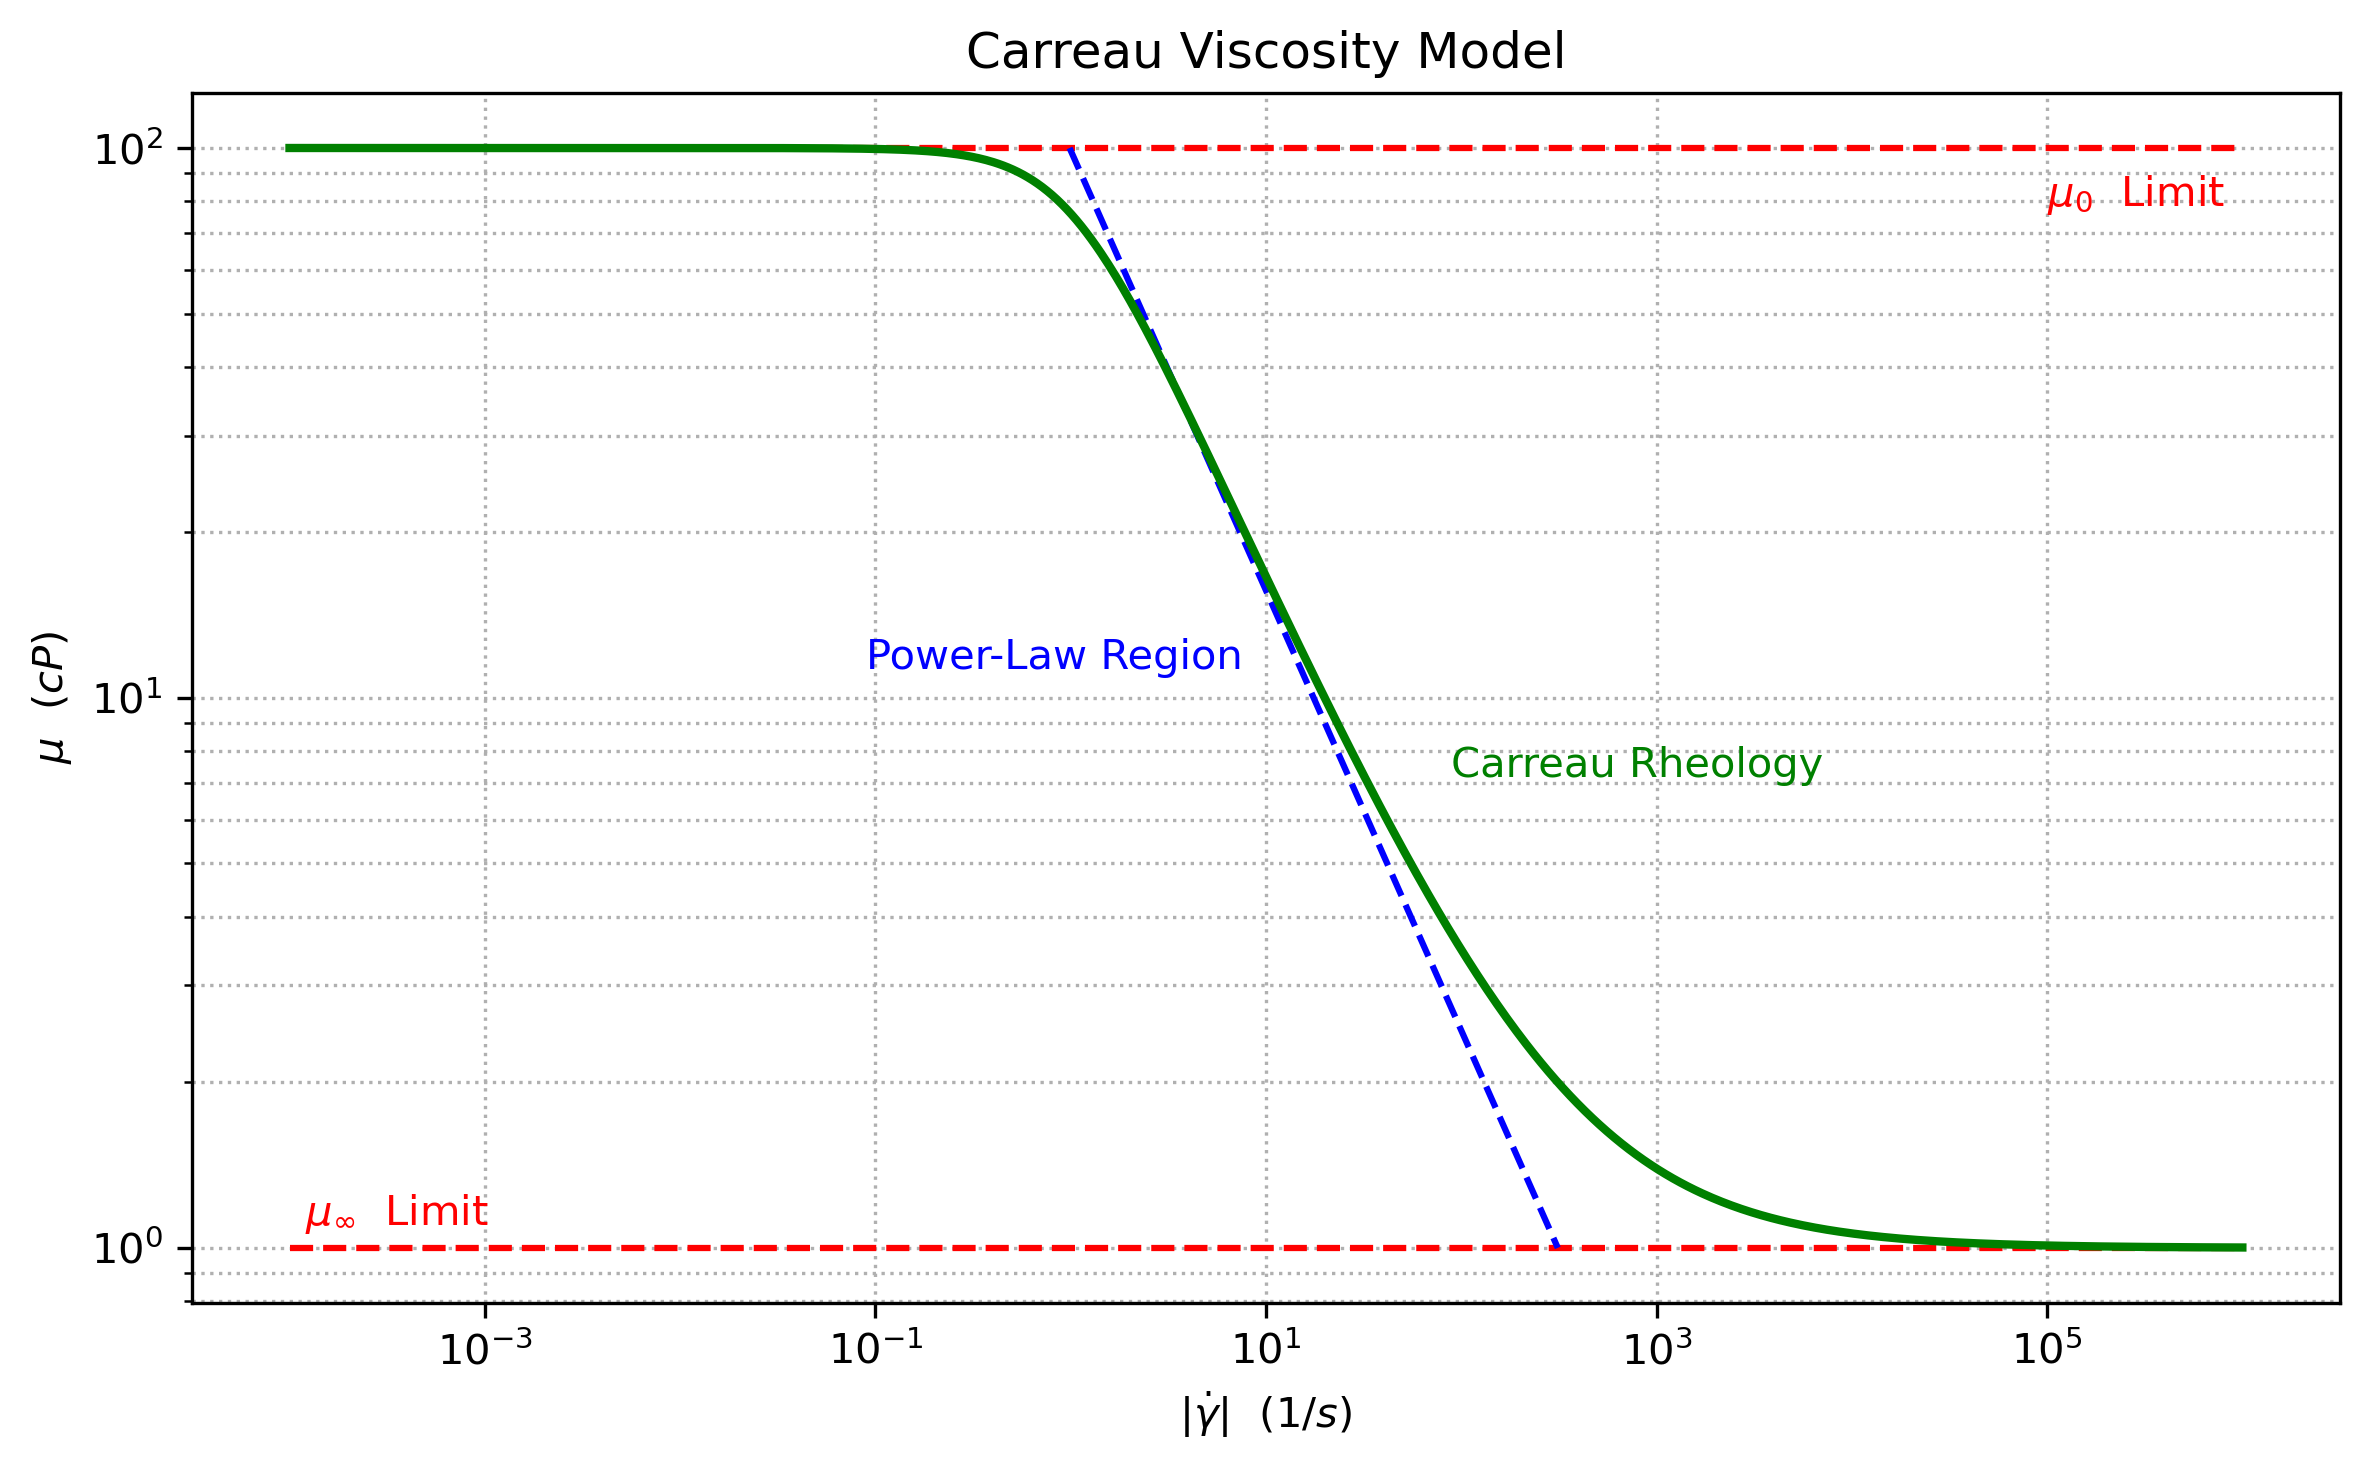
\includegraphics[width=.4\linewidth]{shear_thinning.png}
    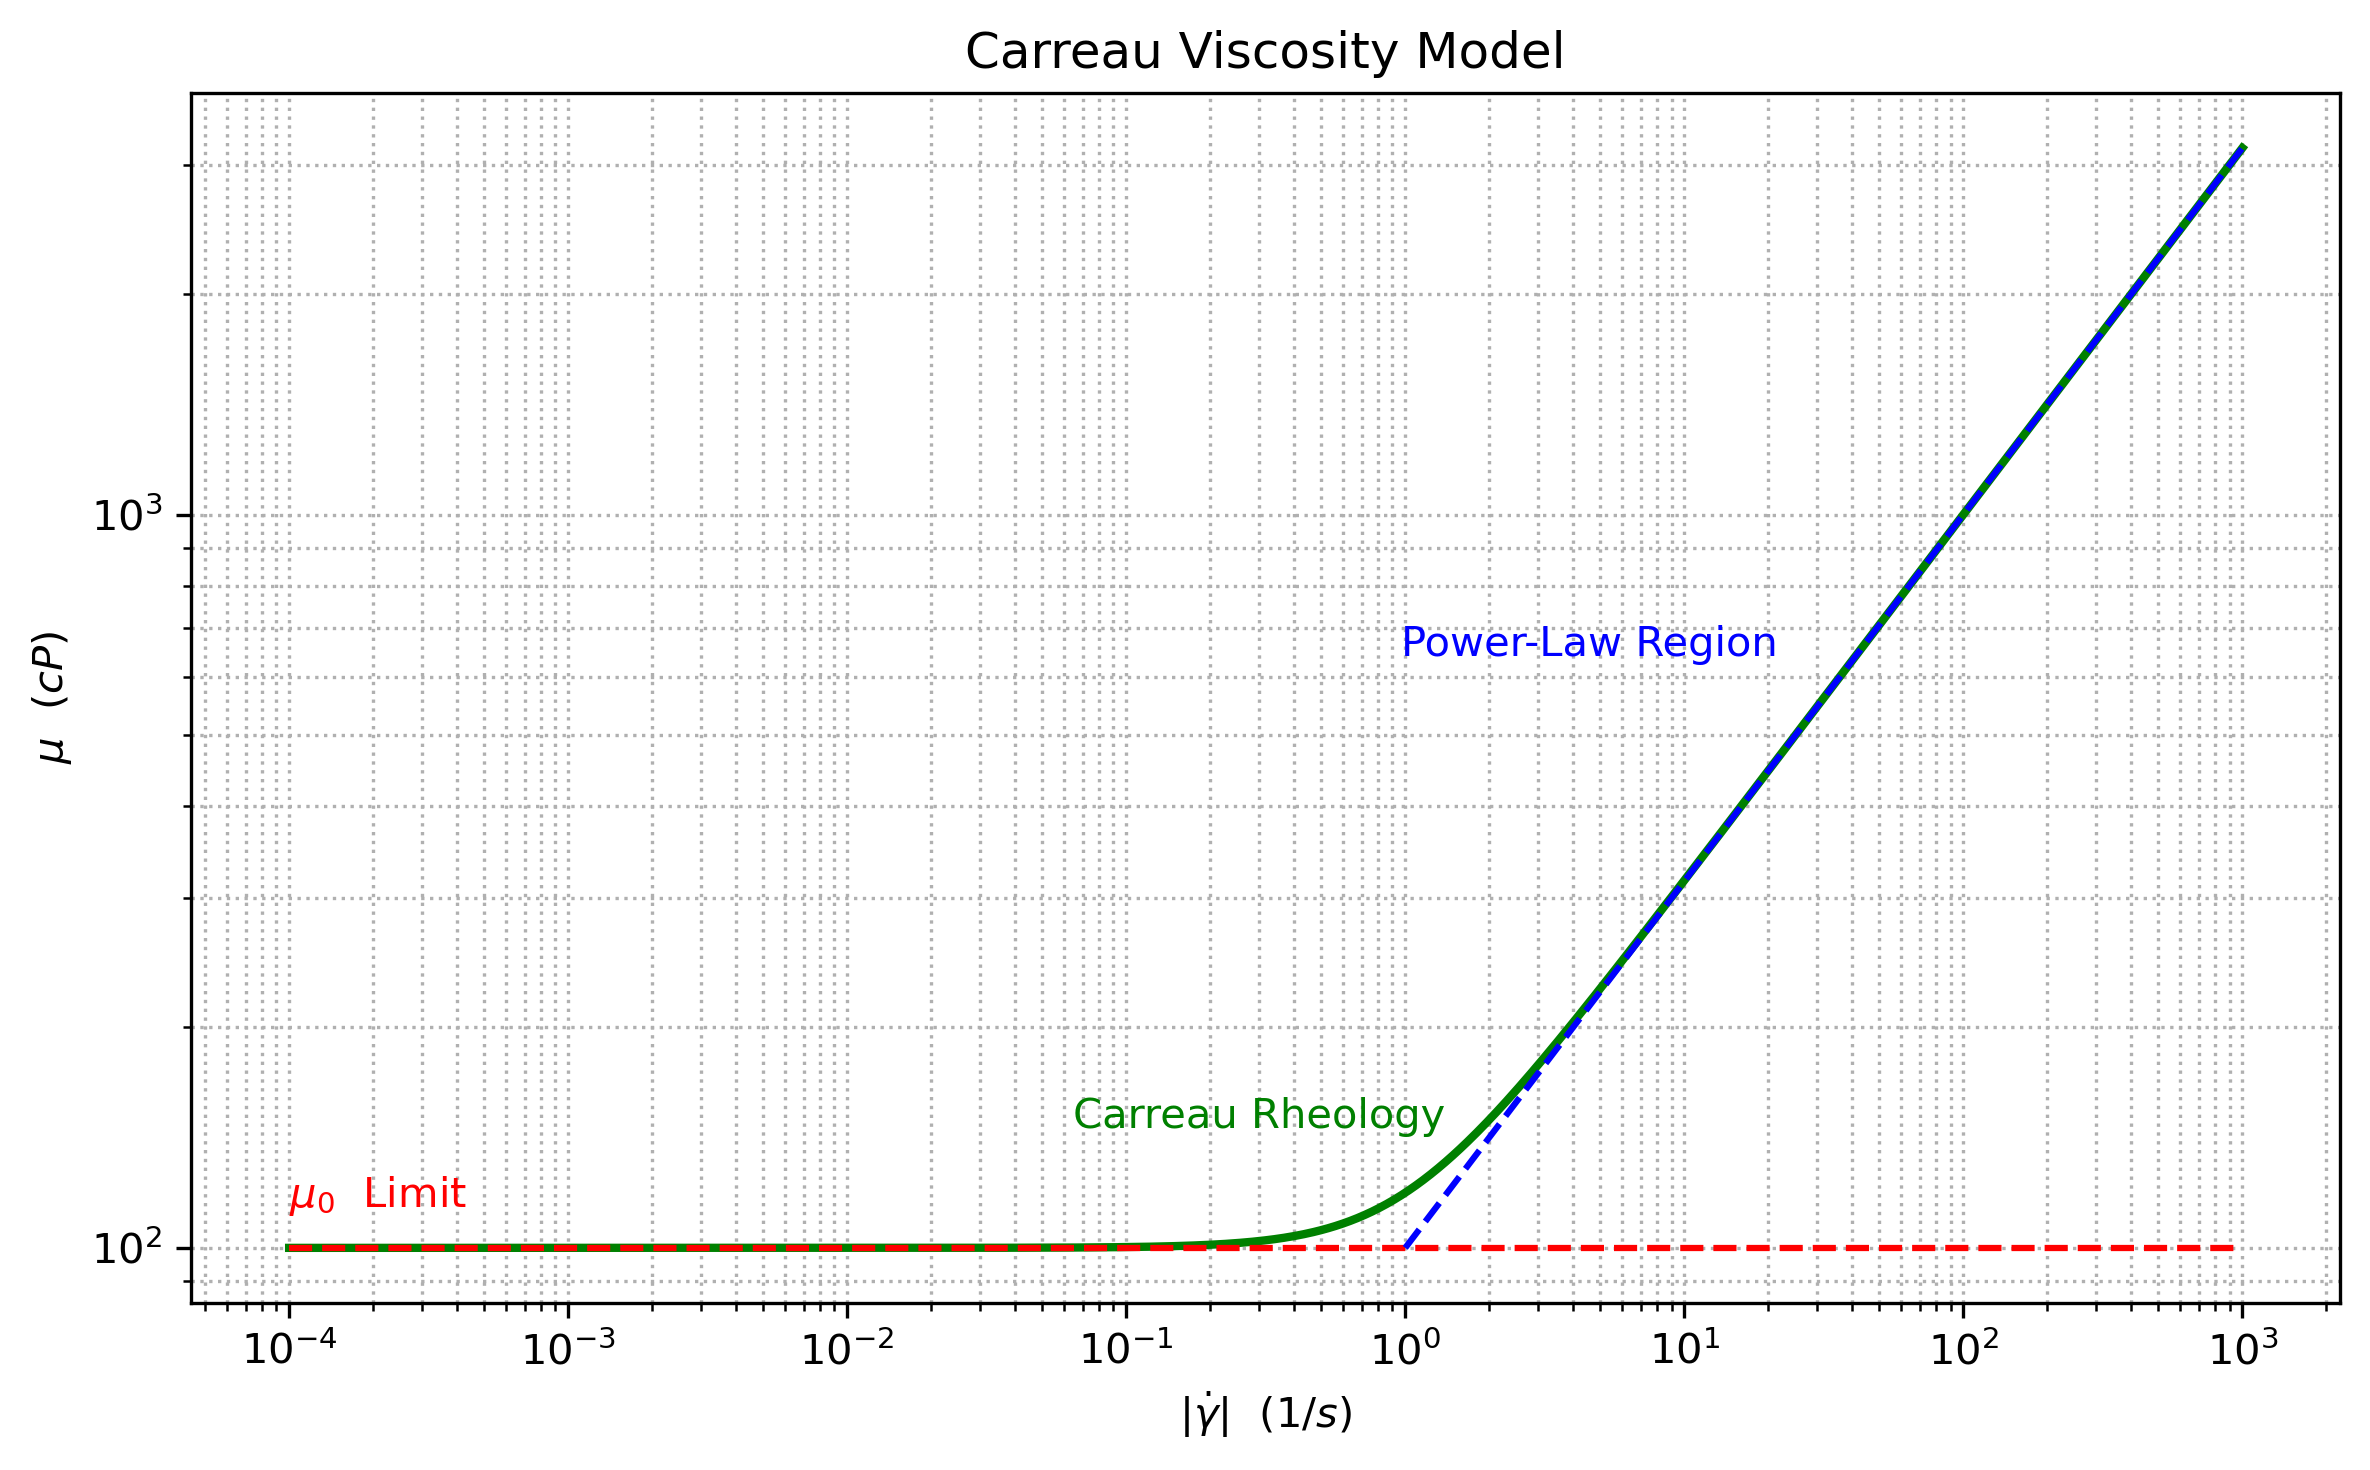
\includegraphics[width=.4\linewidth]{shear_thickening.png}
    \caption{Typical rheological curves showing the dependence of viscosity, $\mu$, on the magnitude of the rate of strain tensor, $|\gd|$.  The power-law region has slope $\alpha-1$ on a log-log plot: a) Shear-thinning behavior; b) Shear-thickening behavior.}
    \label{fig:rheology}
\end{figure}

To address these deficiencies, more realistic generalized viscosity relations---such as the Carreau model---have been used in previous studies of Sakiadis and Blasius boundary layer flows \cite{PANTOKRATORAS, Griffiths}.  The Carreau model incorporates both shear-dependent power-law behavior and its asymptotic Newtonian limits, providing a smooth transition between low-shear and high-shear regimes as shown in Figure~\ref{fig:rheology}; it can thus fully characterize many typical experimentally measured viscosity curves. The Carreau model is expressed as

\begin{equation}
    \mu = \mu_\infty + (\mu_0 - \mu_\infty)\left(1 + (\lambda|\gd|)^2\right)^{(\alpha-1)/2} \label{carreau_full}
\end{equation} where $\mu_0$ is the Newtonian viscosity at low strain-rate magnitudes ($|\gd| \ll 1/\lambda$), $\mu_\infty$ is the Newtonian viscosity at high strain-rate magnitudes ($|\gd| \gg 1/\lambda$), and $\lambda$ is a relaxation time parameter.  In many practical flow fields, the high strain-rate Newtonian plateau is not reached, and rheological data may be well fit by setting $\mu_\infty = 0$. Under these circumstances, the Carreau model becomes \begin{subequations}
\begin{equation}
    \mu = \mu_0\left(1 + (\lambda|\gd|)^2\right)^{(\alpha-1)/2}. \label{carreau_simplified}
\end{equation} From this, it is straightforward to deduce the low-shear and power-law asymptotes shown in Figure~\ref{fig:rheology} as
 \begin{equation} \mu \sim \mu_0 ~~~~(|\gd| \to 0) \hphantom{\sum\sum} \mu \sim \mu_0\lambda^{\alpha-1} |\gd|^{\alpha-1} ~~~~(|\gd| \to \infty). \label{carreau_asymptotes} \end{equation}
The intersection between these asymptotes defines the critical rate of strain, $|\gd|_c$, for the onset of shear thinning as \begin{equation} |\gd|_c = \frac{1}{\lambda}. \label{power_law_carreau_limit}\end{equation} Thus, the parameter $\lambda$ controls the onset of shear thinning through (\ref{power_law_carreau_limit}) (see Figure~\ref{fig:rheology}), and the consistency coefficient $K$ in the limiting power-law model may be expressed in terms of Carreau parameters by comparing (\ref{power_law_carreau_limit}) and (\ref{power_law_constitutive_equation}) as \begin{equation}
    K = \mu_0 \lambda^{\alpha-1}. \label{carreau_power_law_limit_constistency_parameter}
\end{equation} \end{subequations} The connection between the Carreau and power-law models is thus made clear via (\ref{carreau_power_law_limit_constistency_parameter}). Note that the power-law model (\eqref{power_law_constitutive_equation} with \eqref{carreau_power_law_limit_constistency_parameter}) and the Carreau model (\eqref{carreau_full} or \eqref{carreau_simplified}) both reduce to a constant Newtonian viscosity for $\alpha=1$, i.e. \begin{equation}
    \mu = \mu_0 ~~~~\forall ~ |\gd|. \label{newtonian_viscosity}
\end{equation}

The power-law model is often utilized in fundamental research studies to examine phenomenologically how shear-dependent viscosity affects a flow, regardless of its practical range of applicability.  To date, the authors are unaware of any systematic study demonstrating the efficacy of the power-law model in predicting boundary layer flow structure compared with more realistic viscosity models. One feature of more realistic models---such as the Carreau model examined here---is that they do not admit similarity solutions for the Blasius and Sakiadis flows, which complicates both analysis and computation.  One aim of the present work is to assess the extent to which the predictions of simpler, self-similar models provide adequate descriptions of Blasius and Sakiadis flows compared with those using the Carreau model.  To do so, we focus on wall shear as a metric of comparison, but also examine differences in velocity profiles that arise between these models.

The power-law model provides an incomplete description of fluid rheology (again, refer to Figure~\ref{fig:rheology}), and there are some notable changes in the mathematical structure of boundary layer flows that arise upon changing the value of the power-law exponent $\alpha$ in \eqref{power_law_constitutive_equation}.  This change of structure is relevant to our comparative study of power-law and Carreau model results, and we recount some of that literature here.  For Blasius boundary layers, it is well-known that an infinitely differentiable velocity profile is obtained for shear-thinning fluids ($\alpha < 1$), but the velocity profile loses smoothness for shear-thickening fluids ($\alpha>1$): the velocity profile has a discontinuity in its fourth derivative, although it is continuous through its third.  Denier and Dabrowski \cite{Dabrowski} indicate that this discontinuous solution structure arises from a breakdown in the boundary layer equations far from the wall when the viscosity is suitably small.  They demonstrate that a continuous solution can be obtained by introducing a ``viscous diffusion layer" that incorporates viscous derivatives neglected in the boundary layer equation. In this paper, we demonstrate that the Carreau model---a viscosity model with built-in Newtonian limits---yields a continuous solution for all $\alpha$ without the need to invoke modifications to the boundary layer approximation itself.

Previous work on the Sakiadis boundary layer using a power-law model indicates that no solution exists for all shear-thickening fluids ($\alpha > 1$) and for some shear-thinning fluids ($\alpha < 1/2$) \cite{Fox, NonNewtonian}. These results are based on the fact that the dimensionless stream function, $f$, satisfies $\text{d}f/\text{d}\eta \to 0$ as $\eta \to \infty$, where $\eta$ is the similarity variable (corresponding to large distances from the wall). Previous work assumes an asymptotic form $f \sim C + h(\eta)$ where $C$ is a constant and $h(\eta) \ll C$ as $\eta \to \infty$. The claim of no solutions for $\alpha < 1/2$ is based on the fact that this assumption is not self-consistent for $\alpha < 1/2$.  However, in this paper we demonstrate that solutions do exist in the form $f \sim A(\eta + E)^p$, where $A$ and $E$ are constants with $0<p<1$.  Furthermore, solutions do exist for shear-thickening flows ($\alpha > 1$) with $f$ identically constant for $\eta$ sufficiently large, and these solutions are \textit{not} continuously differentiable in their fourth derivative; this structure is analogous to that found in the Blasius problem for a shear-thickening power-law fluid \cite{Zhizhin1978-us, Pavlov1982-qh}. We show that these additional power-law boundary layer solutions yield wall-shear stress predictions that agree with those from the Carreau model at locations along the wall where significant shear-dependent behavior is invoked.

The organization of the paper is as follows. In Section 2, the formulations of the Sakiadis and Blasius problems are provided for Newtonian, power-law, and Carreau model fluids. Although the Carreau constitutive law does not admit a similarity solution, we make use of previous literature \cite{Griffiths} to recover a one-parameter family of ODE solutions that describe the flow at each streamwise location along the wall. In Section 3, we examine the new power-law solutions we have identified for the Sakiadis flow for $\alpha < 1/2$ and $\alpha > 1$. Section 4 presents results showing that the wall shears predicted for a Carreau fluid are well-approximated by those predicted by corresponding Newtonian or power-law similarity solutions, depending on the flow regime, and also provides comparisons of velocity profiles between different viscosity models.  In Section 5, we provide a general discussion on the suitability and limitations of self-similar solutions as models for realistic Carreau behavior, and we provide conclusions in Section 6.


\section{Formulation}

\subsection{Boundary Layer Equations}

\begin{figure}
    \centering
    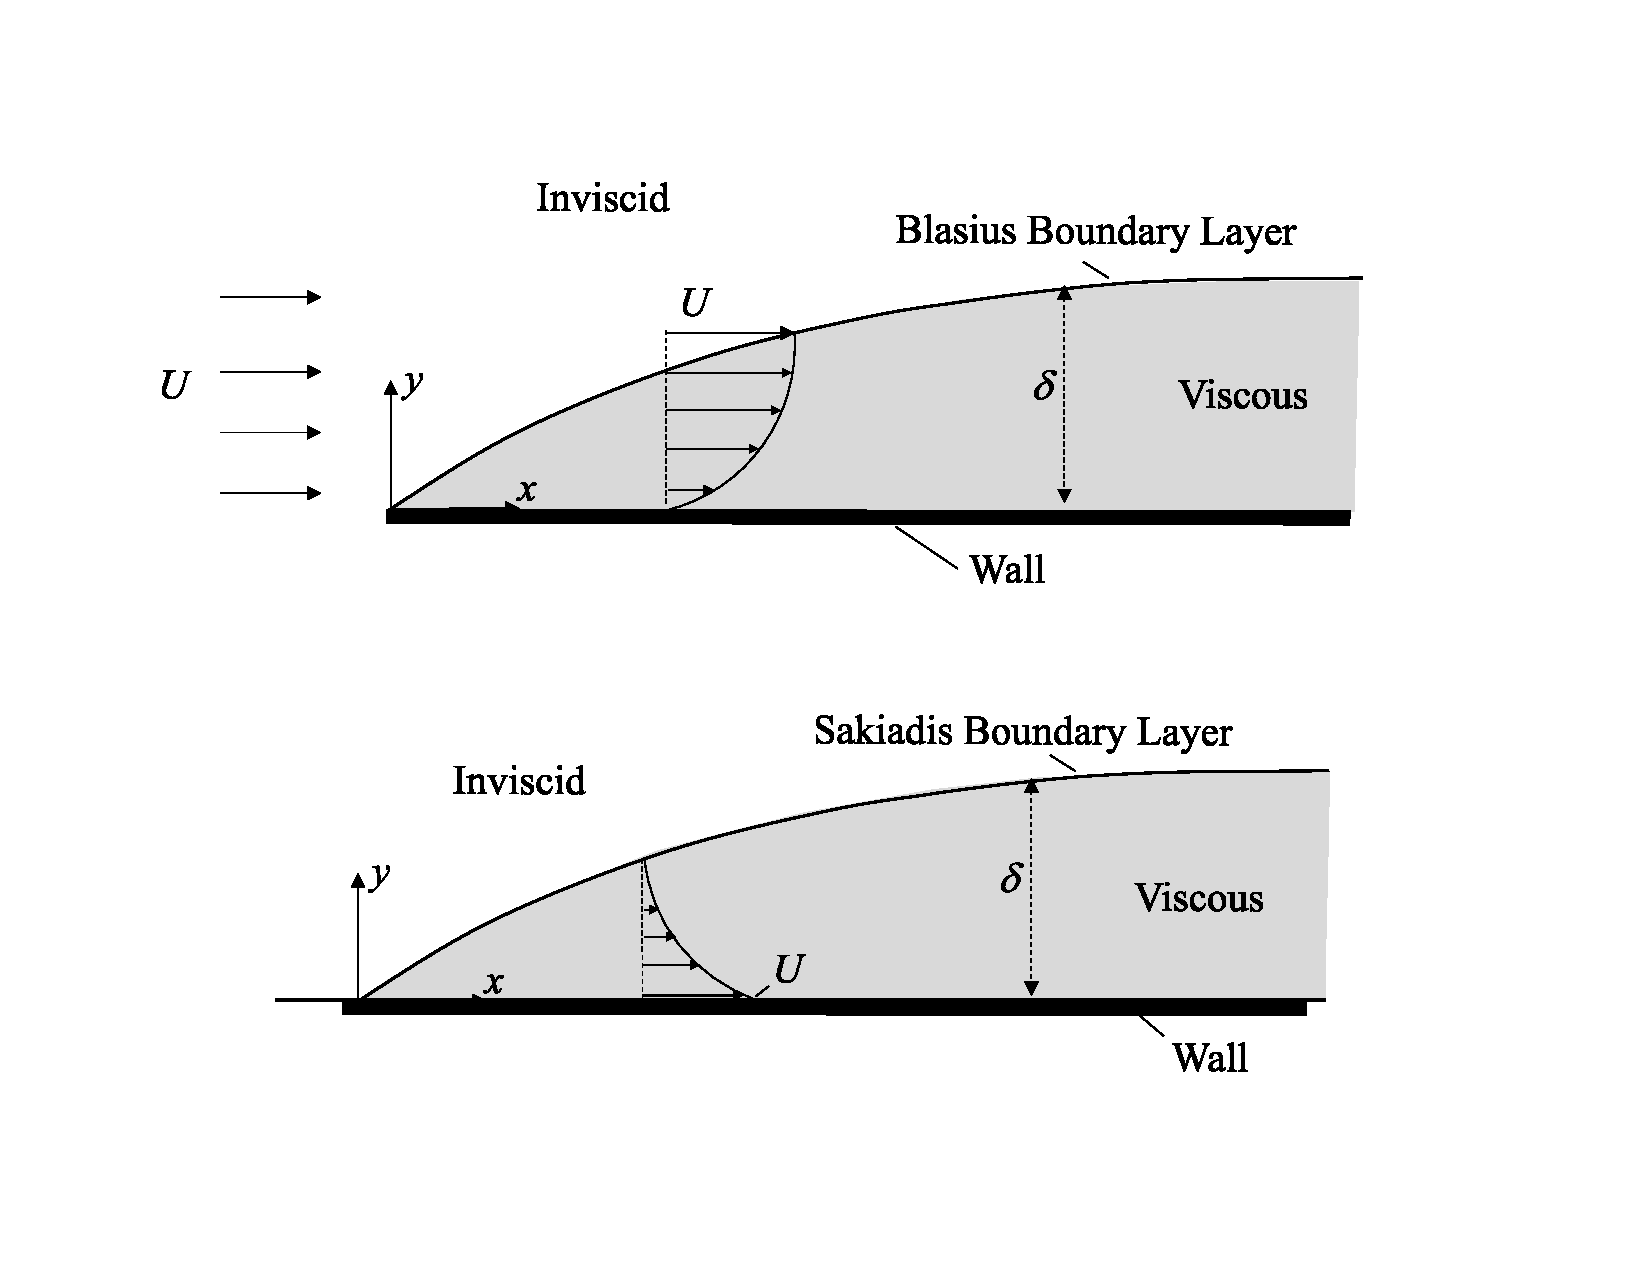
\includegraphics[width=1\linewidth]{sak_stuff.pdf}
    \caption{Configurations for the Sakiadis and Blasius flows.}
    \label{flow_setups}
\end{figure}

We consider the steady boundary layer flow induced by the motion between a fluid and an infinite flat plate (shown in Figure~\ref{flow_setups}). There are two configurations that we examine: the \textit{Sakiadis} boundary layer induced by a moving wall in an otherwise stationary fluid (Figure~\ref{flow_setups}b), and the \textit{Blasius} boundary layer induced by a moving fluid over a stationary wall (Figure~\ref{flow_setups}a). Figure~\ref{flow_setups} shows a schematic of both configurations with the coordinate system and corresponding velocities. Here, the $x$ coordinate is oriented along the wall, the $y$-direction is perpendicular to the wall, and the flow is invariant in the $z$-direction (not shown---oriented out of Figure~\ref{flow_setups}). Corresponding velocities in the $x$ and $y$ directions are $u_x$ and $u_y$, respectively.  In the Blasius configuration, $u_x=U$ is the velocity of the fluid away from the wall ($y \to \infty$); while in the Sakiadis problem, $u_x=U$ is the velocity of the wall ($y=0$).  In both problems, the pressure field is constant and plays no role in the flow dynamics.


In accordance with the boundary layer approximation, the flow in Figure~\ref{flow_setups} is essentially inviscid away from the wall, and the effects of viscosity are confined to a thin region---a boundary layer---near the wall.  As such, velocity variations in the $y$ direction are large compared with those in the $x$ direction, and viscous stresses across the boundary layer dominate.  As a result, the boundary layer form of the equations of motion becomes \cite{Schlichting}

\begin{subequations} \label{blsystem}
    \begin{align}
        &\frac{\partial u_x}{\partial x} + \frac{\partial u_y}{\partial y} = 0 \label{conteqinbl}\\
        & \rho \left\{ u_x \frac{\partial u_x}{\partial x} + u_y \frac{\partial u_x}{\partial y} \right\} = \frac{\partial \tau_{yx}}{\partial y} \label{blmomeq}
    \end{align} where the relevant component of the stress tensor is given as \begin{align}
        \tau_{yx} = \mu \frac{\partial u_x}{\partial y},~~~~\mu = \mu(|\gd|),~~~~|\gd| = \left|\frac{\partial u_x}{\partial y} \right|. \label{stress_tensor_component}
    \end{align} In (\ref{stress_tensor_component}), a generalized Newtonian form for the viscosity $\mu$ has been assumed, as it is a function of the magnitude of the rate of strain as indicated. Consistent with the configurations shown in Figure~\ref{flow_setups}, the boundary conditions are \begin{align}
        \text{Location} && \text{Blasius}~~~~~ && \text{Sakiadis}~~~~~ \nonumber \\
        y = 0 && u_x = 0 ~~~~ u_y = 0 && u_x = U~~~~u_y=0 \\
        y \to \infty && u_x \to U~~~~~ && u_x \to 0.~~~~~
    \end{align} \end{subequations}

In this paper, we consider specific forms of $\mu(|\gd|)$ in (\ref{stress_tensor_component}) for power-law \eqref{power_law_constitutive_equation}, Carreau \eqref{carreau_full} (or \eqref{carreau_simplified}), and Newtonian \eqref{newtonian_viscosity} models.  Regardless of viscosity model, the system (\ref{blsystem}) can be expressed in terms of a streamfunction $\psi$, satisfying $u_x = \partial \psi/\partial y$ and $u_y = -\partial \psi/\partial x$. The equations are then typically further simplified via a similarity transform or PDE solution methods, as discussed below.

\subsection{Power-Law and Newtonian Fluids}

For a power-law fluid, the PDE system (5) admits a similarity solution using the substitutions \begin{subequations}
    \begin{equation}
        \eta = y\left(\dfrac{\rho U^{2-\alpha}}{Kx}\right)^{1/(\alpha+1)}
    \end{equation}
    \begin{equation}
        f_p(\eta; \alpha) = \frac{\eta \psi}{Uy}
    \end{equation}
\end{subequations} that yields an ODE for $f_p$ given by \begin{subequations} \begin{align}
    & \alpha(\alpha+1)f_p''' + f_pf_p''|f_p''|^{1-\alpha} = 0 \label{power_law_ode_only} \\ &(\mathrm{Blasius})~~~~f_p(0; \alpha)=0~~~~f_p'(0; \alpha)=0~~~~f_p'(\infty; \alpha) \to 1  \\
    & (\mathrm{Sakiadis})~~~~f_p(0; \alpha)=0~~~~f_p'(0; \alpha)=1~~~~f_p'(\infty; \alpha) \to 0 \label{power_law_sak_bcs}
\end{align} \label{power_law_ode_general} \end{subequations} The associated streamwise velocity component, $u_x$, may be extracted as \begin{equation} u_x = U \frac{\partial f_p}{\partial \eta}. \label{streamwise_velocity_expression} \end{equation}The dimensional expression for the wall shear rate for a power-law fluid, $\tau_p$, is likewise extracted from the solution for $f_p$, and is expressed as \begin{subequations} \begin{equation}
    \tau_p = K \left(U \left|f_p''(0; \alpha)\right|\left(\dfrac{\rho U^{2-\alpha}}{Kx} \right)^{1/(\alpha+1)}  \right)^\alpha \label{pl_dimensional_wall_shear}
\end{equation} In (\ref{pl_dimensional_wall_shear}), note that $f_p''(0; \alpha)<0$ for the Sakiadis flow, and $f_p''(0; \alpha)>0$ for the Blasius flow. The analogous expressions for a Newtonian fluid can be obtained from (\ref{pl_dimensional_wall_shear}) by inserting $\alpha=1$ and $K=\mu_0$ in accordance with \eqref{power_law_constitutive_equation} to yield \begin{equation}
    \tau_n = |f_n''(0)| \sqrt{\dfrac{\rho \mu U^3}{x}} \label{newtonian_dimensional_wall_shear}
\end{equation} \end{subequations} where the subscript $n$ denotes the Newtonian wall shear rate, and $f_n(\eta) = f_p(\eta; 1)$.

\subsection{Carreau Fluid}

\hspace{\parindent} The boundary layer equations for a Carreau fluid do not admit a self-similar solution as they do for Newtonian and power-law fluids. In general, this necessitates a numerical solution of the governing PDE system \eqref{blsystem} (using $\mu$ in \eqref{carreau_full}) for Blasius or Sakiadis configurations. However, following the approach of \cite{Griffiths}, one can transform the governing system into an ODE via the similarity variable used for a Newtonian fluid.  In this form, the $x$-dependence does not disappear completely, but arises solely as a parameter in the problem.  This necessitates that the ODE be solved at each streamwise location $x$.

As such, we define a dimensional streamfunction for the Carreau model, $f_c$, as\begin{equation} f_c = \psi \sqrt{\dfrac{\rho}{\mu_0 x U}}\end{equation} and the similarity coordinate \begin{equation} \eta = y \sqrt{\dfrac{\rho U}{\mu_0 x}}.\end{equation} Substituting (10) and (11) into (5), one obtains not a single ODE as in the self-similar case, but an ODE with an $x$-dependent parameter. Defining the local parameter $\delta$ as \begin{equation}
    \delta = \frac{\lambda^2 U^3 \rho}{\mu_0 x}, \label{delta_definition}
\end{equation}  \begin{subequations} and writing \begin{equation} \bar{\mu}_\infty = \mu_\infty / \mu_0,\end{equation} $f_c$ satisfies
    \begin{align}
        \left\{\bar{\mu}_\infty + (1-\bar{\mu}_\infty)\left[1+\alpha\delta \left(\frac{\mathrm{d}^2f_c}{\mathrm{d}\eta^2}\right)^2 \right] \left[1+\delta \left(\frac{\mathrm{d}^2f_c}{\mathrm{d}\eta^2}\right)^2 \right]^{(\alpha-3)/2} \right\}\frac{\mathrm{d}^3f_c}{\mathrm{d}\eta^3} + \frac{1}{2}f_c \frac{\mathrm{d}^2f_c}{\mathrm{d}\eta^2} = 0 \label{carreau_ode_form_ode} &\\ (\mathrm{Blasius})~~~~f_c(0; \alpha)=0~~~~f_c'(0; \alpha)=0~~~~f_c'(\infty; \alpha) \to 1  \label{carreau_ode_form_blasius_bcs} & \\
    (\mathrm{Sakiadis})~~~~f_c(0; \alpha)=0~~~~f_c'(0; \alpha)=1~~~~f_c'(\infty; \alpha) \to 0 \label{carreau_ode_form_sakiadis_bcs} &
    \end{align} \label{carreau_ode_form_full_system}
\end{subequations}

For given rheological parameters, the ODE system (\ref{carreau_ode_form_full_system}) has a single parameter, $\delta$, that changes with distance $x$ downstream (Figure~\ref{flow_setups}). Thus, by solving the system (\ref{carreau_ode_form_full_system}) for an appropriate array of $\delta$ values spanning the desired $x$-domain of interest, the whole flow field may be determined without considerable computational effort. As indicated in \eqref{delta_definition}, the $x$-dependent parameter $\delta$ incorporates the constant $\lambda$ present in the Carreau viscosity model \eqref{carreau_full}.  It is apparent from the location of $\delta$ in (\ref{carreau_ode_form_ode}) that it acts as an effective relaxation time---the inverse relationship with $x$ indicates that the magnitude of shear-dependent behavior decreases downstream.  This observation is physically intuitive, as it is consistent with the physics of a growing boundary layer in the original $x$-$y$ domain (Figure~\ref{flow_setups}), and indicates that velocity gradients decrease accordingly, thus reducing the degree of shear-dependent behavior.

It is often the case that $\mu_\infty$ is not reached in practice. Although the approach that follows does not require $\bar{\mu}_\infty=0$, we neglect it for clarity of presentation. For $\mu_\infty=0$, the dimensional expression for the wall shear for the Carreau model \eqref{carreau_full} is \begin{equation}
    \tau_{c} = \sqrt{\dfrac{\rho  \mu_0U^3}{ x}}f_c''\left(0; \delta\right)\left(1 + \delta f_c''\left(0; \delta\right)^2  \right)^{(\alpha-1)/2} .\label{carreau_wall_shear_dimensional_expression}
\end{equation}

To solve the relevant boundary value problems for power-law (and therefore Newtonian, for $\alpha=1$) or Carreau rheologies from Sections 2.2 and 2.3, we convert the relevant boundary value problems (\ref{power_law_ode_general}) and (\ref{carreau_ode_form_full_system}) into initial value problems by imposing a value of $f_c''(0, \delta)$.  We then truncate the domain to a length $L$, and use RK4 with shooting to meet the $y\to\infty$ boundary conditions in \eqref{carreau_ode_form_sakiadis_bcs}---now imposed at $y=L$. The domain length is then increased and the calculation repeated until convergence is achieved to within an absolute error tolerance of $10^{-6}$.

\section{New Sakiadis Solutions for Power-Law Fluids}

\hspace{\parindent} To facilitate comparison with the Carreau model solution for Blasius and Sakiadis flows, the self-similar solution to the ODE (\ref{power_law_ode_general}) for a power-law fluid is necessary. Power-law solutions for Blasius flows are well-known for all values of $\alpha>0$. For the case of a Sakiadis flow, however, \cite{Fox} and \cite{NonNewtonian} indicated that no solutions exist for two distinct classes of power-law fluids: those with $\alpha < 1/2$ and $\alpha > 1$. This conclusion is based on an analysis of one particular asymptotic form of the Sakiadis flow away from the wall. In what follows, we show that alternative asymptotic forms are possible, which enables power-law solutions to be obtained in these previously excluded regimes of $\alpha$.

\subsection{Shear-Thinning Fluids ($\alpha < 1/2$)}


We begin with a discussion of solutions for shear-thinning fluids.  In the Blasius case, it is known that a solution to the power-law Blasius equation exists for all $\alpha < 1$ with the property that $f \sim \eta$ as $\eta \to \infty$. In the Sakiadis case, however, the existence of a power-law solution is only known for $\alpha \in (1/2, 1]$.  Given the similarities between the ODEs governing Blasius and Sakiadis flows, this inability to obtain a power-law solution outside of this range is not anticipated.  We resolve this non-analogous behavior in what follows.

For a Sakiadis flow, the dimensionless streamfunction $f_p(\eta; \alpha)$ satisfies (\ref{power_law_ode_only}) with boundary conditions (\ref{power_law_sak_bcs}). The Newtonian Sakiadis equation ($\alpha=1$) admits a solution having asymptotic behavior that can be derived assuming $f_p(\eta; 1) \to C$ and using the method of dominant balance \begin{equation} f_p(\eta; 1) \sim C + Ge^{-C\eta/2} ~~ (\eta \to \infty)\end{equation} with $C$ and $G$ constants \cite{GenMeth}. For shear-thinning fluids with $1/2 < \alpha < 1$, an analogous dominant balance subject to the same assumption yields \begin{equation}
    f_p\left(\eta; \frac{1}{2} < \alpha < 1\right) \sim C + D\left(1 + E\eta \right)^{^{\frac{2\alpha-1}{\alpha-1}}} ~~ (\eta \to \infty), \label{sakiadis_shear_thinning_classical_asymptotic}
\end{equation} with $C, D$, and $E$ constants; as is standard for dominant balance problems, these constants remain arbitrary when only the asymptotic behavior is assessed. Note that this form breaks the dominant-balance assumption for $\alpha < 1/2$, when the leading constant term $C$ becomes asymptotically subdominant to the second term, which grows as $\eta \to \infty$ for $\alpha < 1/2$. The conclusion that there is no solution for $\alpha<1/2$ in \cite{Fox} and \cite{NonNewtonian} is based on the asymptotic form (\ref{sakiadis_shear_thinning_classical_asymptotic}); in what follows, we show that another dominant balance can be satisfied that leads to an expanded range of admissible $\alpha$ values.

In particular, the boundary condition (\ref{power_law_sak_bcs}) does not require \textit{a priori} that $f_p \sim C$ as $\eta \to \infty$. Rather, a solution to equation (\ref{power_law_ode_only}) that satisfies equation (\ref{power_law_sak_bcs}) admits the asymptotic form \begin{subequations} \begin{equation}
    f_p\left(\eta; 0 < \alpha < \dfrac{1}{2} \right) \sim H \left(\eta+J\right)^{p} ~~ (\eta \to \infty),
\end{equation} where \begin{equation} p = \dfrac{1-2\alpha}{2-\alpha} \end{equation}  and \begin{equation}
    H = \left(\dfrac{\alpha(\alpha+1)(2-p)}{p^{1-\alpha}(1-p)^{1-\alpha}}\right)^{^{\frac{1}{2-\alpha}}}.
\end{equation} \label{power_law_sakiadis_new_asymptotic} \end{subequations} \noindent In (\ref{power_law_sakiadis_new_asymptotic}), $J$ is an arbitrary constant that reflects the autonomous nature of the ODE (\ref{power_law_ode_general}).  One may write $f_p''(0)=\kappa$ and vary the initial condition $\kappa$ to examine $f'$ as $\eta \to \infty$. In so doing, we find that for $\kappa$ greater than a critical value $\kappa=\kappa_p$, solutions for $f_p$ are monotonically increasing for all $\eta \geq 0$, while they are nonmonotone and eventually decrease with $\eta$ for $\kappa<\kappa_p$. Figure~\ref{fig:shooting} shows this structure, indicating that the solution corresponding to $\kappa=\kappa_p$ is a separatrix delineating the two asymptotic behaviors. At $\kappa=\kappa_p$, the solution smoothly approaches $f_p' \to 0$ as $\eta \to \infty$. This value of $\kappa_p$ is the unique solution with this property, and we propose it represents the correct solution for $\alpha<1/2$.

\begin{figure}
    \centering
    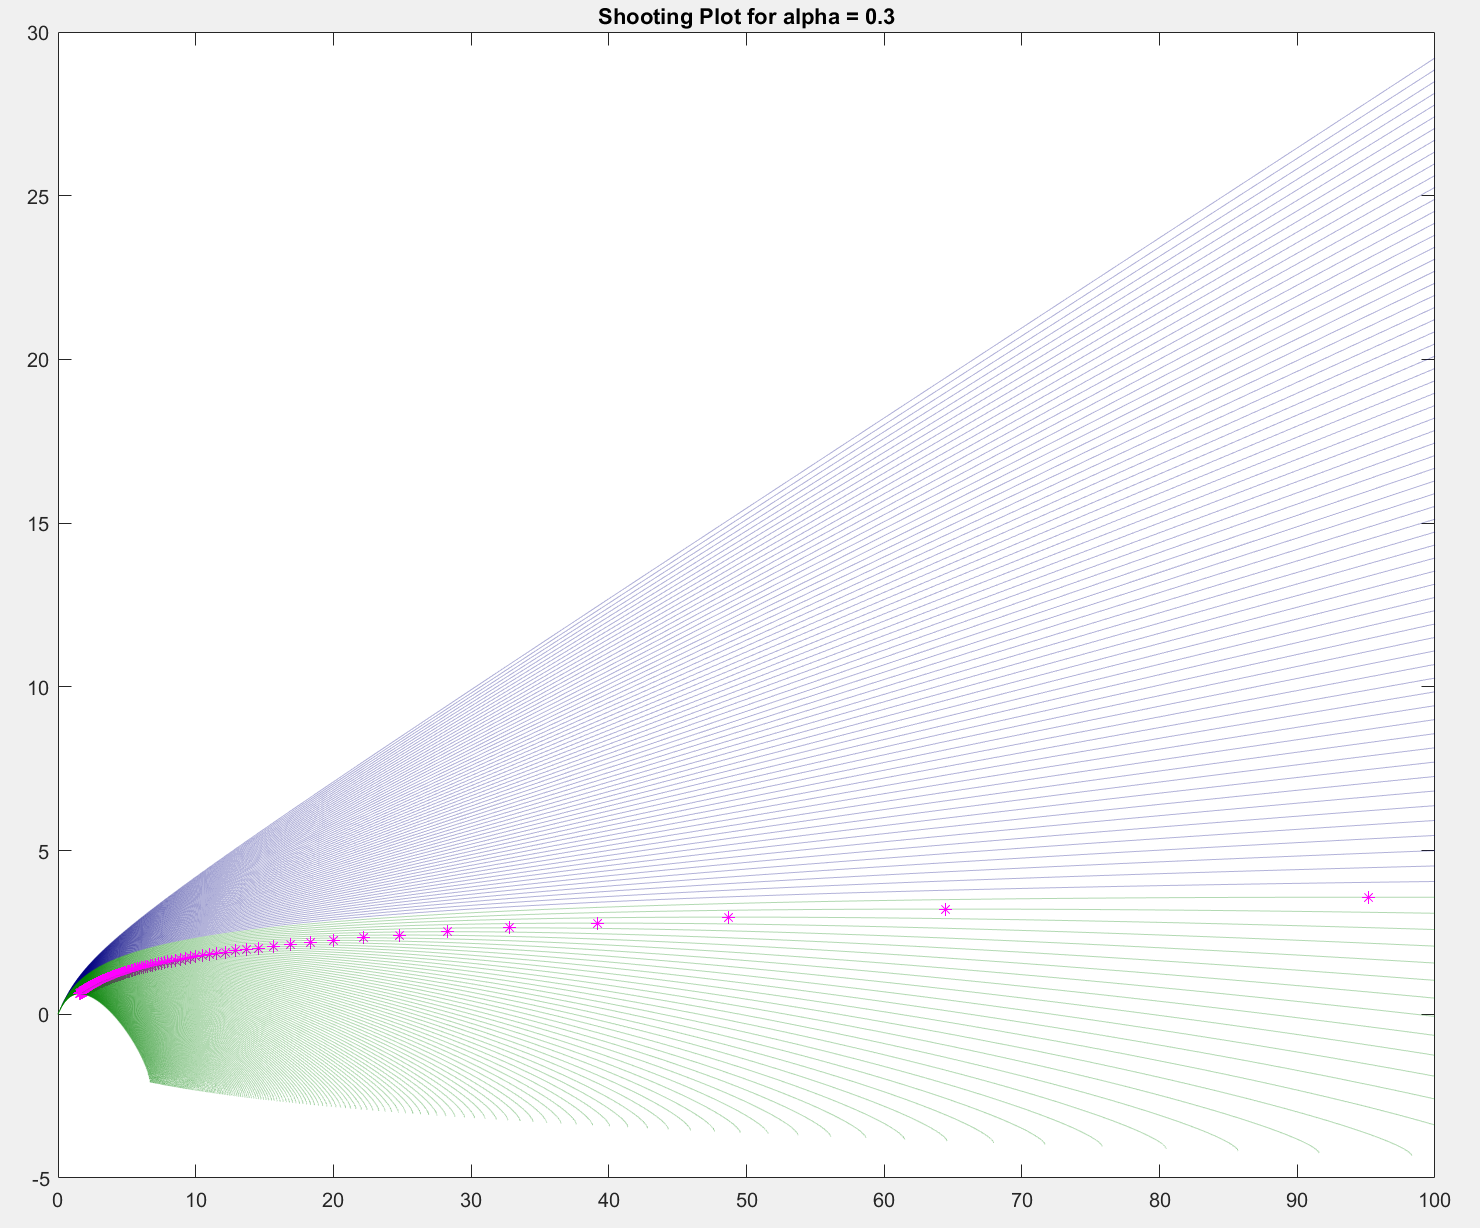
\includegraphics[width=0.6\linewidth]{shooting_fixed.png}
    \caption{Shooting showing convergence to the separatrix solution with domain lengthening for the shear-thinning Sakiadis flow with $\alpha < 1/2$. Solutions above the separatrix orbit are shown in blue, and solutions below it are shown in green; the latter obtain a local maximum in $\mathbb{R}^+$.}
    \label{fig:shooting}
\end{figure}

The separatrix solution is found numerically to match the asymptotic behavior (\ref{power_law_sakiadis_new_asymptotic}). Figure~\ref{fig:new_asymptotic} illustrates the log-log structure of this new asymptotic regime, confirming the power-law growth $f_p \sim H(\eta + J)^p$ predicted by (\ref{power_law_sakiadis_new_asymptotic}) for representative values of $\alpha < 1/2$. Furthermore, numerical results confirm that the solution to the power-law Sakiadis equation yields a computed value of $\kappa_p$ that closely follows the high-shear limit for wall shear observed in the Carreau model, to be described in Section 4. Taken together, the consistency of the wall-shear rate and asymptotic behavior predictions with Carreau predictions justifies the conclusion that a new admissible Sakiadis power-law solution has been found for $\alpha<1/2$.

\begin{figure}
    \centering
    
\includegraphics[width=0.6\linewidth]{new_thinning_asymptotic.png}
    \caption{Log-log plot of the separatrix solution $f_p(\eta; \alpha)$ for the shear-thinning Sakiadis boundary layer for representative values of $\alpha < 1/2$. The dashed lines show the predicted asymptotic form $f_p \sim H(\eta + J)^p$ from (\ref{power_law_sakiadis_new_asymptotic}), confirming the new power-law growth regime.}
    \label{fig:new_asymptotic}
\end{figure}

\begin{figure}
    \centering
    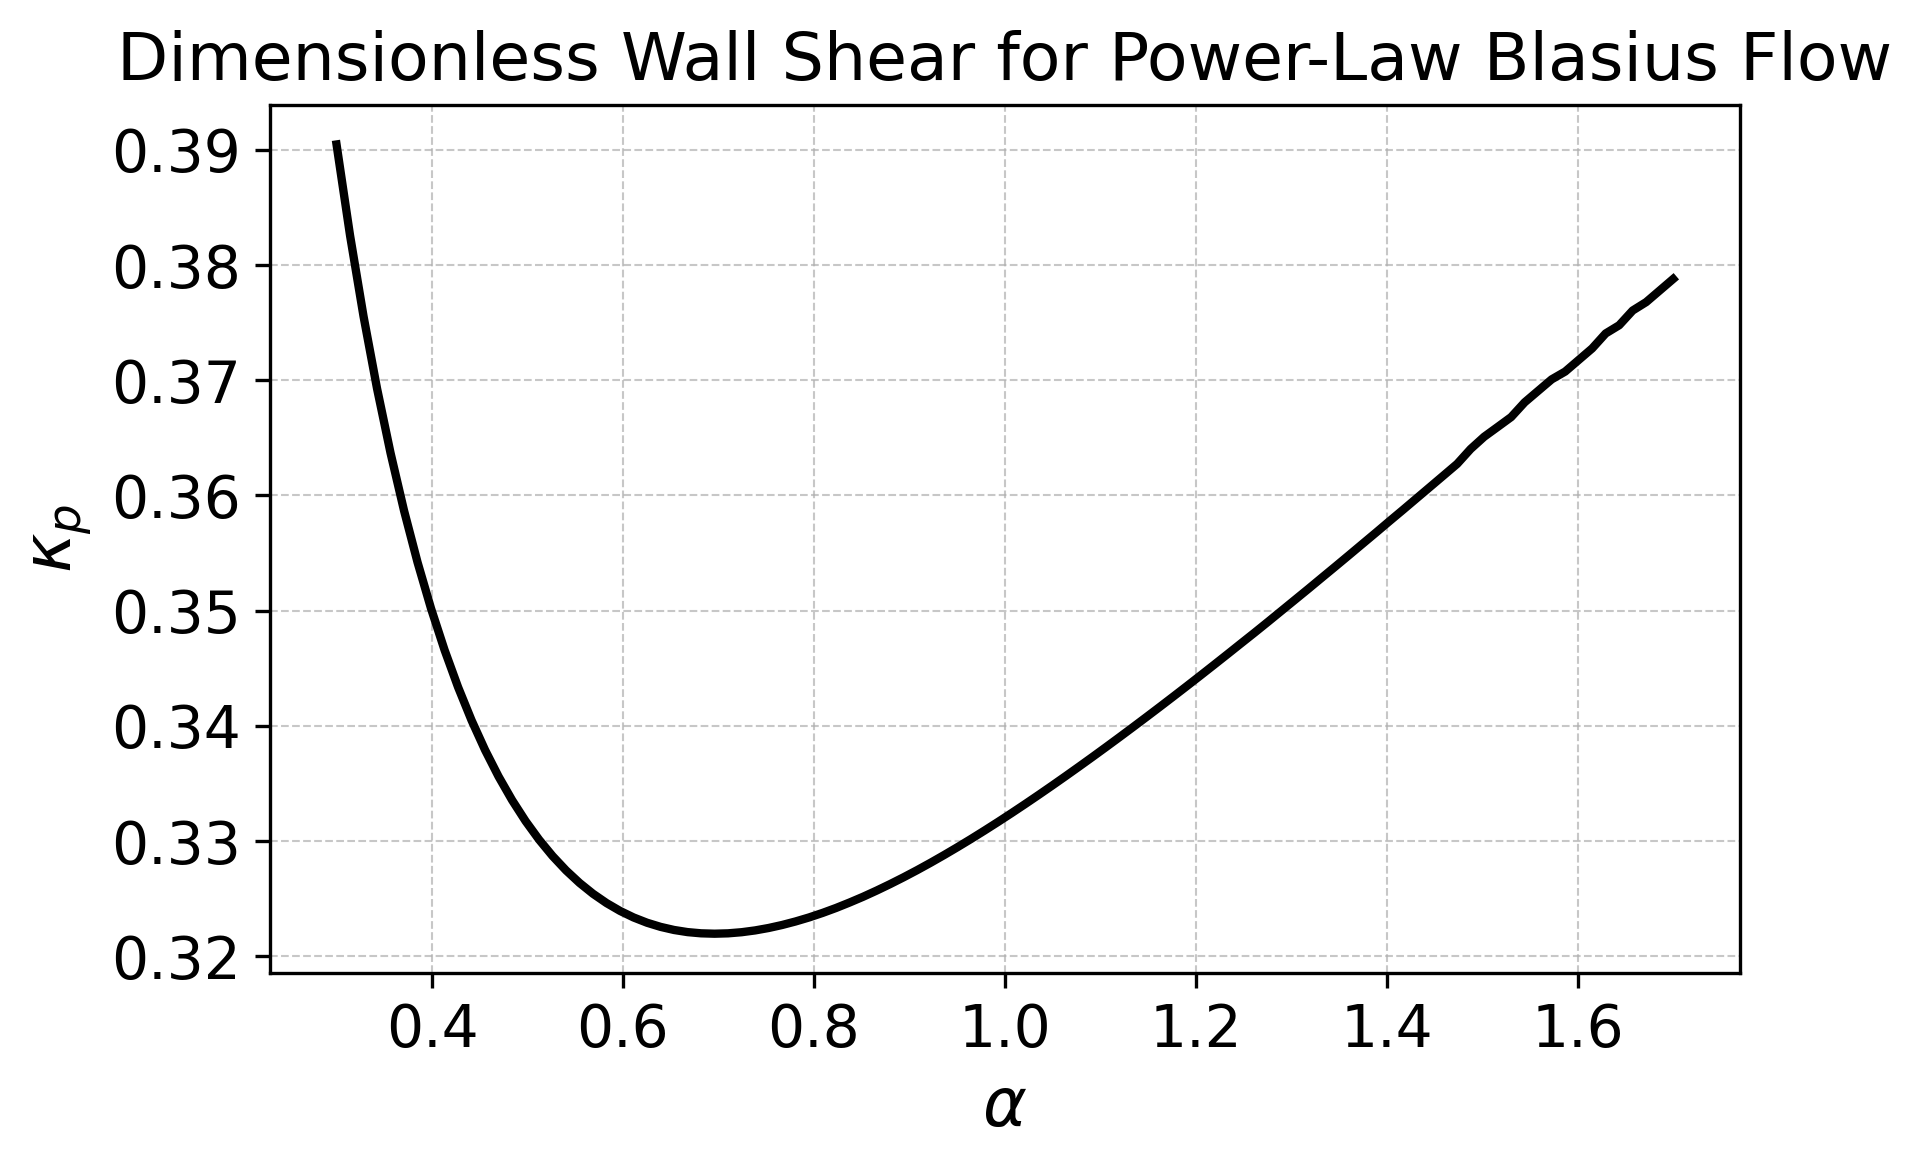
\includegraphics[width=\textwidth]{pl_blas_kappa.png}
     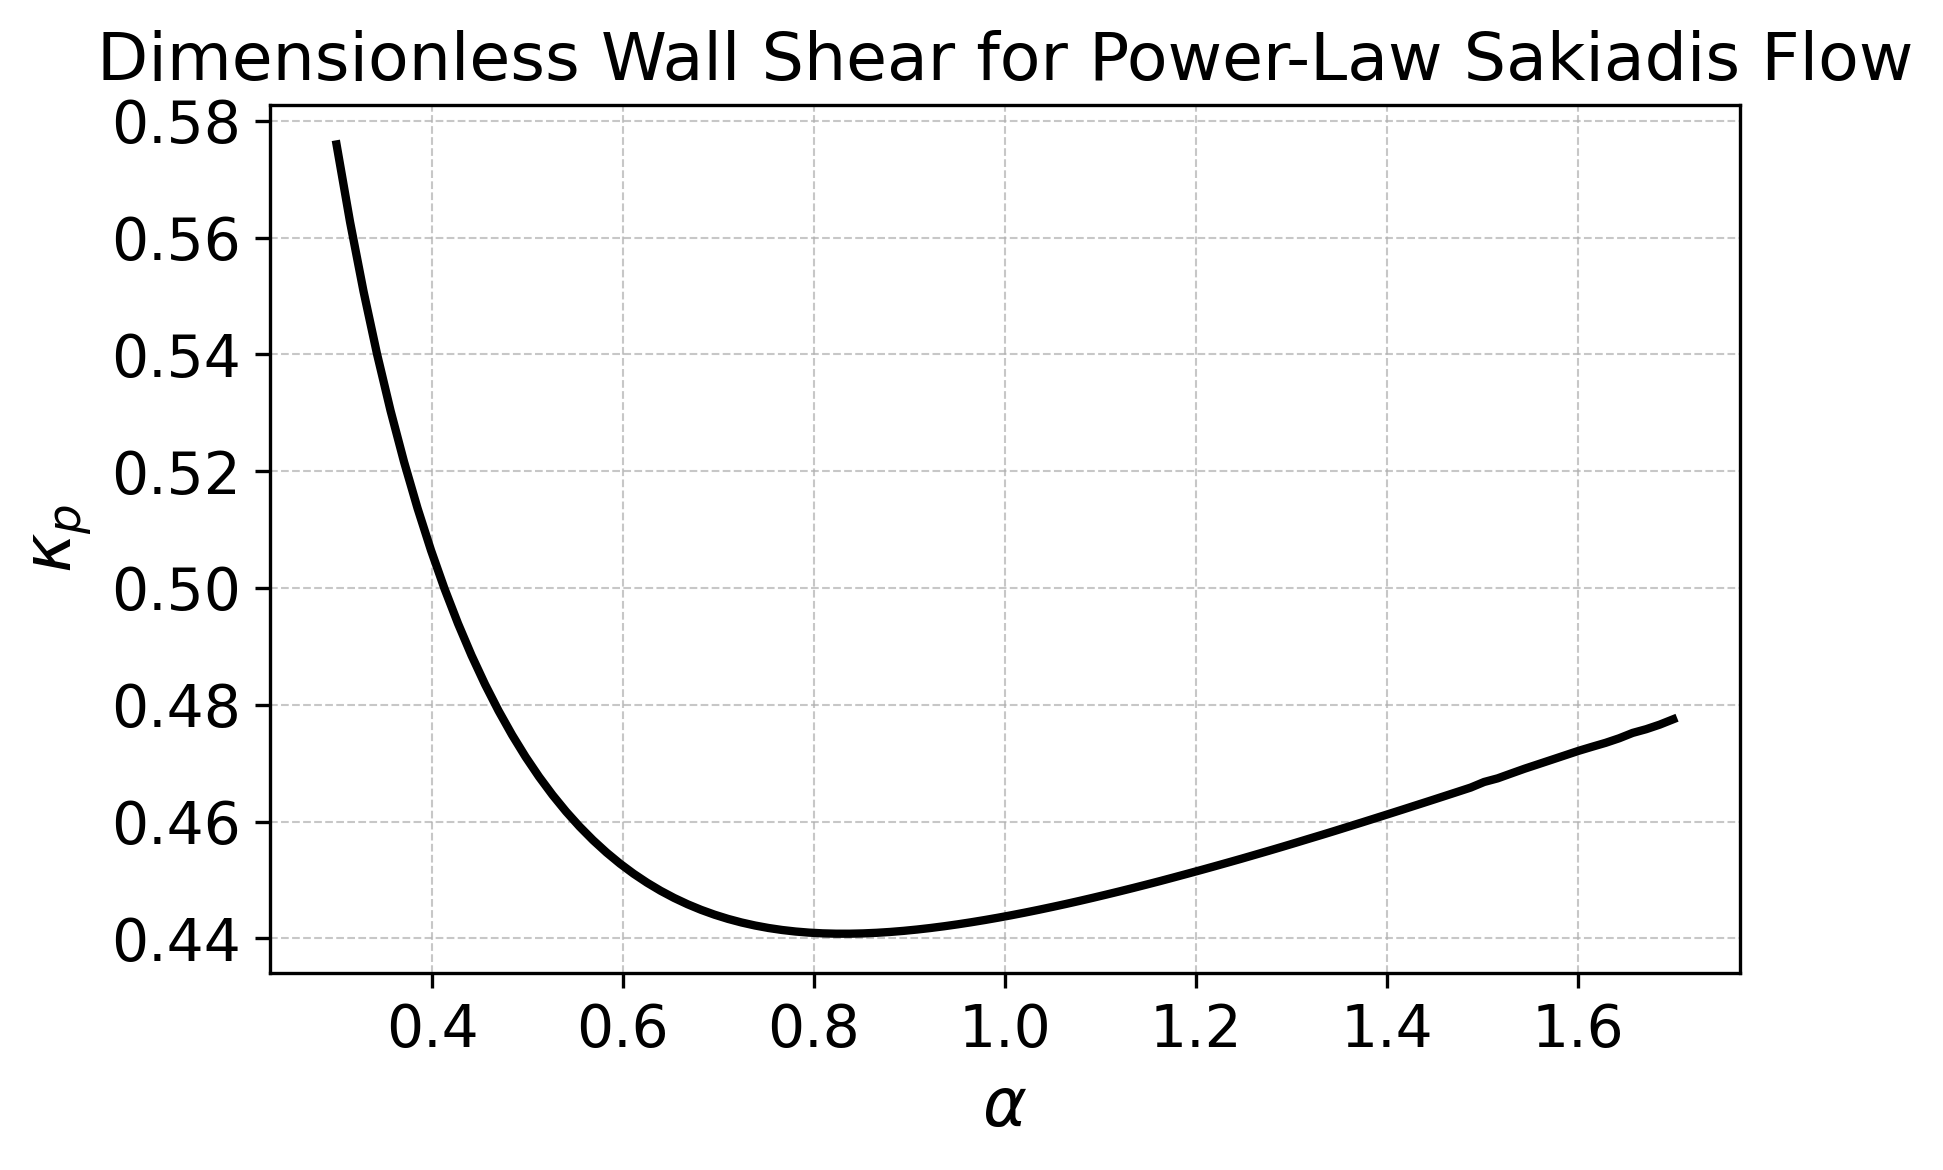
\includegraphics[width=\textwidth]{pl_sak_kappa.png}
    \caption{Nondimensional power-law wall shear coefficient $\kappa$ as a function of $\alpha$ for the Blasius boundary layer (top) and Sakiadis boundary layer (bottom).}
    \label{fig:kappavsalpha}
\end{figure}

% The case $\alpha = 0$ is physically nonsensical, so this treatment gives the structure of all shear-thinning Carreau fluids except in the case that $\alpha = 1/2$. In this case, we conjecture that \begin{equation} f_p\left(\eta; \dfrac{1}{2}\right) \sim D \log(\eta) ~~ (\eta \to \infty), \end{equation} This is a natural guess because for $\alpha > 1/2$, $f$ goes to a constant asymptotically, and for $\alpha < 1/2$, $f$ goes to a small power asymptotically, meaning $f$ likely limits to a function that grows slower than any power but increases faster than a constant. While this is far from a complete demonstration, we find it likely that $f_p(\eta; 1/2)$ admits a logarithmic solution.


\subsection{Shear-Thickening Fluids ($\alpha > 1$)}

\hspace{\parindent} When $f_p \to C$ is also assumed for shear-thickening ($\alpha>1$) power-law fluids, the asymptotic equation (\ref{sakiadis_shear_thinning_classical_asymptotic}) arises, again indicating that no solution satisfies the dominant balance, since the second term is not subdominant to the first \cite{Bender}. However, in this case we once again find that there exists another class of power-law solutions. Insight can be gained here by analogy to the well-known structure of the Blasius problem. For a power-law fluid in the Blasius boundary layer, it is known that the dimensionless streamfunction admits a ``singular solution'' that is $C^4$ but not $C^5$ (four but not five times continuously differentiable) at a distinguished ``singular'' point along the solution curve \cite{Zhizhin1978-us, Pavlov1982-qh}. We note that, unlike the shear-thinning case (where the ODE (\ref{power_law_ode_only}) is not Lipschitz), in the shear-thickening regime the ODE is Lipschitz, so the usual existence and uniqueness theorem (Picard--Lindel\"{o}f) applies, and the singular behavior must arise from a different mechanism.

For this flow, it is found that there exist constants $C_1$ and $C_2$ such that the solution satisfies $f_p(\eta; \alpha) = C_2$ for all $\eta \geq C_1$. Thus, according to \eqref{streamwise_velocity_expression}, the streamwise velocity $u_x$ is identically zero (plug flow with no relative motion) for $\eta \geq C_1$. For $\eta<C_1$, the solution to the boundary layer equation (\ref{power_law_ode_general}) applies in its full form. At $\eta=C_1$, the velocity, its gradient, and the velocity profile curvature are all continuous and satisfy (\ref{power_law_ode_only}), but the fourth derivative of $f_p$ is discontinuous. Figure~\ref{fig:thickbest} shows this discontinuity structure in the fifth derivative for a representative shear-thickening case. Because of the scaling properties of the Sakiadis equation, choosing any $f_p''(0)=\kappa$ and solving (\ref{power_law_ode_only}) as an IVP will still yield this structure.

We claim the situation for the Sakiadis boundary layer is analogous to that of the Blasius case; to our knowledge, this is the first time that this structure has been proposed for the Sakiadis problem. A ``finite-width'' solution to the power-law boundary layer equation exists, having the property that outside of a bounding region above the plate, the fluid velocity is exactly zero. Near the plate, the boundary layer behaves according to the solution of (\ref{power_law_ode_general}); at the edge of the boundary layer, there is a discontinuous fourth derivative in $f_p$, but the velocity, its gradient, and the profile curvature are continuous and satisfy (\ref{power_law_ode_only}). Similarly to the shear-thinning case, numerical results indicate a separatrix solution exists between monotone and nonmonotone solutions, yielding a structure analogous to Figure~\ref{fig:shooting}; here, however, the streamfunction becomes identically constant at a finite value of $\eta$ (rather than growing as $\eta \to \infty$ as happens for $\alpha<1/2$) when $\kappa=\kappa_p$. This structure gives, it seems, the unique $C^3$ solution to (\ref{power_law_ode_general}) for $\alpha > 1$, and yields values of $\kappa_p$ that agree with the high-shear limit in the Carreau model.

\begin{figure}
    \centering
    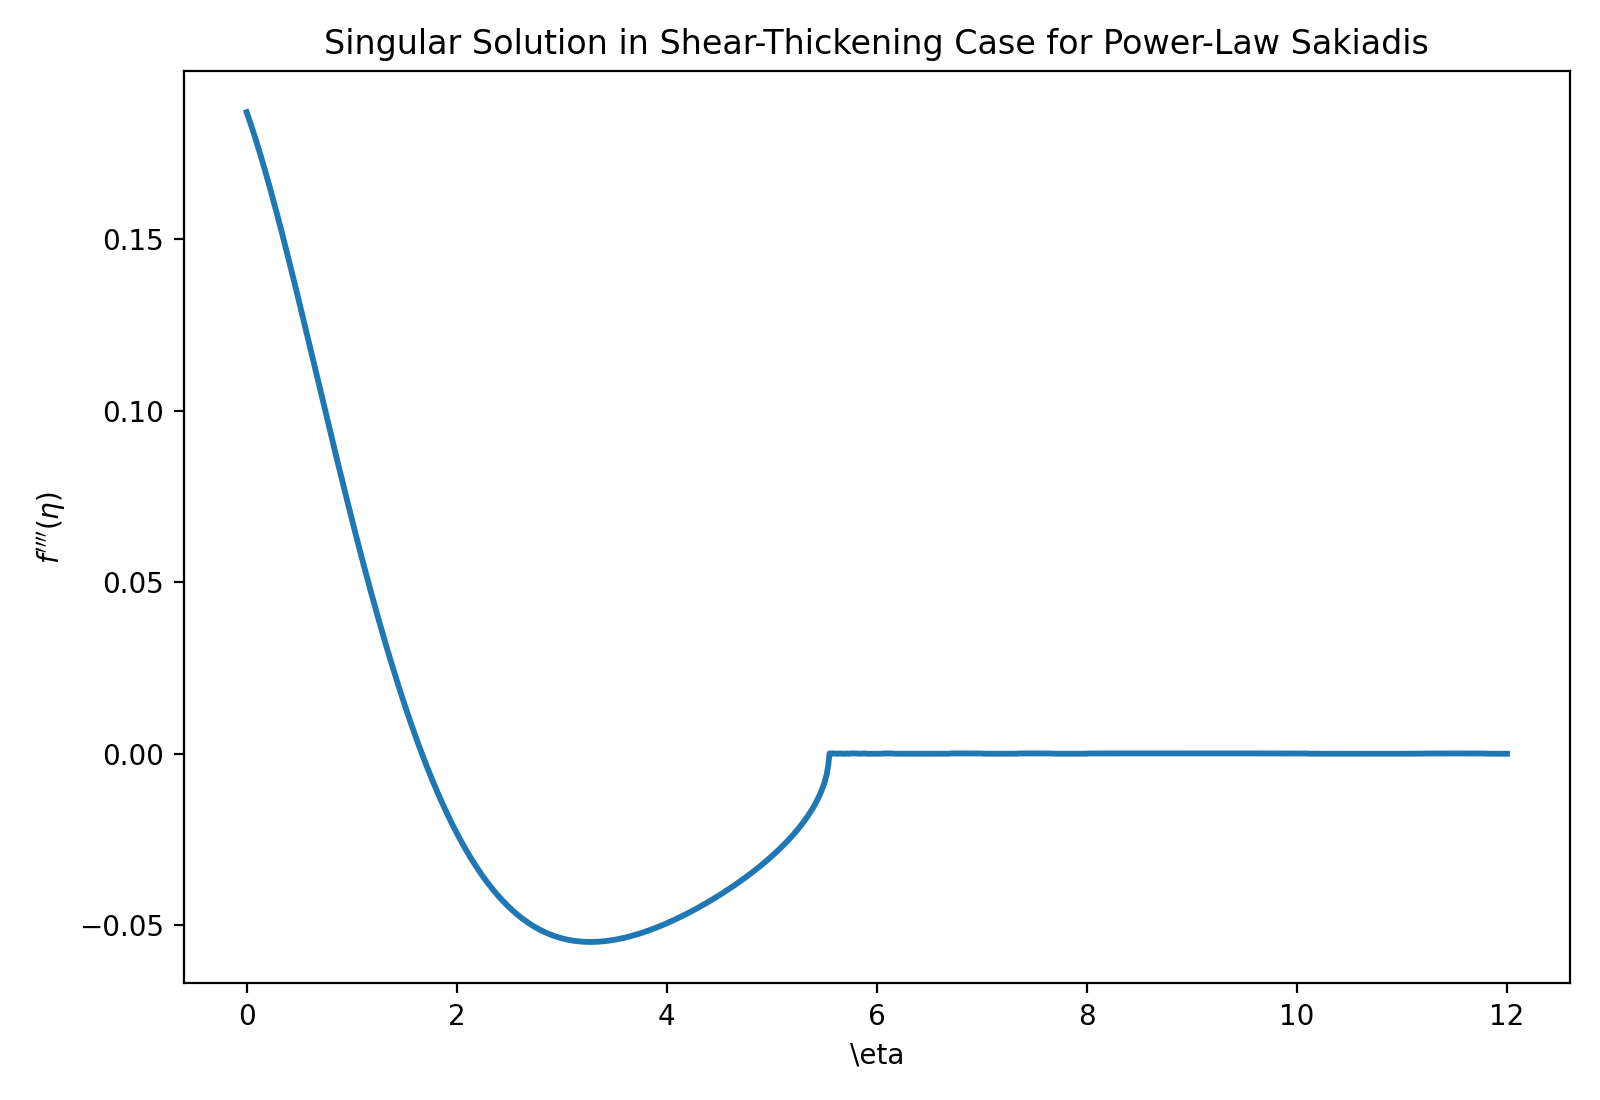
\includegraphics[width=0.5\linewidth]{thick_best.png}
    \caption{Discontinuity in the fifth derivative for the new power-law solution in the shear-thickening Sakiadis case.}
    \label{fig:thickbest}
\end{figure}


\section{Power-Law/Newtonian Models vs.\ Carreau Prediction for Wall Shear}

\subsection{Direct Comparison of Wall Shear}

We compare wall shear rate predictions for Newtonian, power-law, and Carreau fluids in dimensionless form.  To do so, we express these wall shear expressions ((\ref{pl_dimensional_wall_shear}), (\ref{newtonian_dimensional_wall_shear}), and (\ref{carreau_wall_shear_dimensional_expression})) in dimensionless form using Newtonian scalings. Denoting dimensionless quantities with an overbar, we write \begin{equation}
    \bar{\tau}_i = \dfrac{\tau_i}{\rho U^2} \hphantom{\sum\sum} \mathrm{for}~~i=n, c, p
\end{equation} For a Newtonian fluid with viscosity $\mu_0$, we have that \begin{equation}
    \bar{\tau}_n = \kappa_n \operatorname{Re}_{n, x}^{-1/2}, ~~~~\kappa_n = f_p''(0; 1), \label{newtwsexpnondim}
\end{equation} where the local Reynolds number is given by \begin{equation} \operatorname{Re}_{n, x} = \rho xU/\mu_0. \label{newtonian_reynolds_number}\end{equation}

For a power-law fluid, the dimensionless wall shear is expressed as \begin{equation}
    \bar{\tau}_p = \kappa_p^\alpha \operatorname{De}^{(\alpha-1)/(\alpha+1)} \operatorname{Re}_{n, x}^{-\alpha/(\alpha+1)}, ~~~~ \kappa_p = f_p''(0; \alpha),  \label{plwsexpnondim}
\end{equation} where $\operatorname{De}$ is the Deborah number given by \begin{equation}
    \operatorname{De} = \frac{\rho \lambda U^2}{\mu_0}.
\end{equation} In writing (\ref{plwsexpnondim}), note that we have utilized the relation $K=\mu_0 \lambda^{\alpha-1}$ to relate the parameter $K$ to the Carreau parameters.

Moreover, using the Newtonian scaling, the nondimensional Carreau wall shear is given by \begin{equation} \bar{\tau}_{c} = \kappa_{c} \operatorname{Re}_{n, x}^{-1/2} \left( 1 +  \kappa_c^2 \frac{\operatorname{De}^2}{\operatorname{Re}_{n, x}} \right)^{(\alpha-1)/2}, ~~~~ \kappa_c=f_c''(0; \delta), \label{carwsexpnondim}\end{equation} where $\operatorname{Re}_{n,x}$ is the local Newtonian Reynolds number as in (\ref{newtonian_reynolds_number}).

Figure~\ref{fig:wallshearfig} shows typical comparisons of local wall shear predictions for Sakiadis and Blasius flows for shear-thinning fluids (top row) and shear-thickening fluids (bottom row).  Note that for small dimensionless distances down the wall (small $\operatorname{Re}_{n, x}$), the power-law model predictions agree with those of the Carreau model; for larger distances, the Newtonian model is in agreement.  As indicated, the power-law and Newtonian predictions serve as asymptotes to the Carreau curve in each regime.

\subsection{Comparison of Wall Shears for Different Models}

By the equations of Section 4.1, we may directly compare the wall shear expressions for different models as a function of the Newtonian Reynolds number $\operatorname{Re}_{n, x}$ and nondimensional Deborah number $\operatorname{De}$. The generic behavior is that for low Reynolds number, near the front of the plate where shear rates are high, the wall shear approaches the power-law limit. The wall shear is in this case a power-law function of the Reynolds number as per (\ref{plwsexpnondim}), corresponding to a straight line on a log-log plot. Further along the plate, where shear rates are lower, the fluid is approximately Newtonian, and the wall shear approaches the Newtonian limit that scales with Reynolds number to the $-1/2$ power as per (\ref{newtwsexpnondim}). The wall shear for a Carreau fluid roughly follows the power-law behavior near the front of the plate until the power-law line intersects the Newtonian asymptote; beyond this transition, the Carreau wall shear closely matches the associated Newtonian prediction.

\begin{figure}
    \centering
    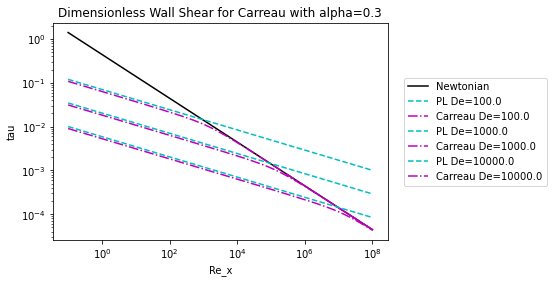
\includegraphics[width=0.4\linewidth]{wallshearsmall.png}
    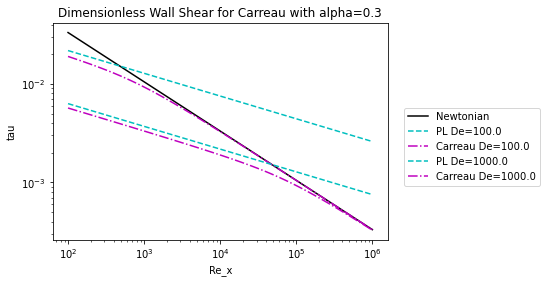
\includegraphics[width=0.4\linewidth]{blas_shear_1.png}
    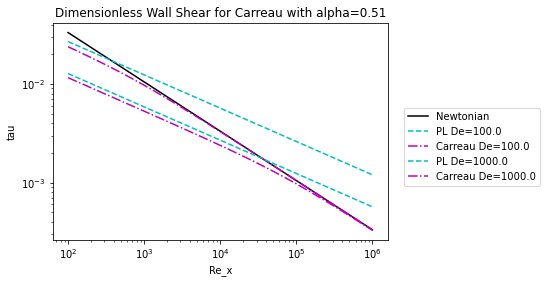
\includegraphics[width=0.4\linewidth]{blas_shear_2.png}
    \caption{Wall shear for Sakiadis (top left) and Blasius (top right, bottom) boundary layers for different power-law exponent $\alpha$ and Deborah number $\operatorname{De}$.}
    \label{fig:wallshearfig}
\end{figure}

\section{Discussion}

\subsection{Limiting Analyses}

One can see that in the shear-thinning case, for high values of strain rate, $\delta$ is small and the expression (\ref{carwsexpnondim}) approaches (\ref{newtwsexpnondim}), showing very concretely that the wall shear behavior of the Carreau model approaches that of a Newtonian fluid in this limit. Note that the behavior of (\ref{carwsexpnondim}) when $\delta$ is large enough to place the flow in the power-law regime requires more careful analysis: although the fluid physically behaves like a power-law fluid, the approach to (\ref{plwsexpnondim}) cannot be easily extracted from the present nondimensionalization without rescaling in accordance with the power-law regime. Numerical results clearly confirm, however, that (\ref{carwsexpnondim}) does recover the power-law behavior in the large $\delta$ regime.

Indeed, for an arbitrary Carreau fluid, we note that sufficiently far along the wall (where the shear is low), the non-self-similar Carreau wall shear is in good agreement with the self-similar prediction for a corresponding Newtonian fluid. For points close to the front of the wall, in the power-law regime, the Carreau wall shear is also well-approximated by the predictions of a power-law fluid.

The transition region between these behaviors is found to occur where the relevant wall shear curves intersect. Because those power-law and Newtonian wall shear curves require no non-self-similar computation, this means one can determine directly which regime is relevant to a particular location along the flow of a Carreau fluid using only intersection information from self-similar flows, without solving the method-of-lines system for the Carreau streamfunction. Setting (\ref{plwsexpnondim}) equal to (\ref{newtwsexpnondim}), this crossover is found to occur at a critical value of $\delta$, denoted $\delta^*$, which is related to $\kappa_n$ and $\kappa_p$ (both functions of $\alpha$) as \begin{equation} \delta^* = \left(\dfrac{\kappa_p^\alpha}{\kappa_n}\right)^{2\frac{1+\alpha}{1-\alpha}}.\end{equation}

We note that $\kappa_p$ varies with $\alpha$ in a way that is tabulated in Figure~\ref{fig:kappavsalpha}, and Figure~\ref{fig:kappacar} shows the corresponding Carreau wall shear coefficient $\kappa_c$ as a function of $\delta$. Over the entire range of $\alpha$ from $0$ to $2$, $\delta^*$ itself changes only from approximately 14 to 20, meaning that the critical value of $\delta$ is of order unity when the crossover between the power-law and Newtonian regimes occurs. This has the following physical interpretation. The applied shear in the boundary layer scales as the wall speed, $U$, divided by the characteristic boundary-layer width, which in the Newtonian case goes as $\sqrt{\nu_0x/U}$. The applied shear thus scales like $U/\sqrt{\nu_0x/U}$. The condition $\delta \sim 1$ can be rearranged to give \begin{equation} \dfrac{U}{\sqrt{\nu_0x/U}} \sim \dfrac{1}{\lambda}. \end{equation} So, to order of magnitude, the crossover between the Newtonian and power-law regions occurs when the applied shear is on the order of the reciprocal relaxation time $1/\lambda$, which is consistent with the typical interpretation of $\lambda$ in the Carreau viscosity model. Since we can compute $\kappa_p$ precisely, however, we also know the crossover location along the boundary layer to a much greater degree of precision for any particular $\alpha$.

\begin{figure}
    \centering
    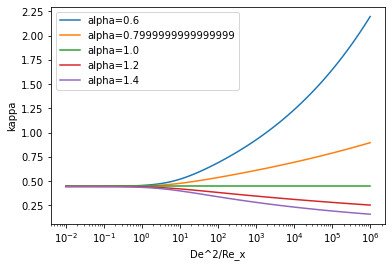
\includegraphics[width=0.45\linewidth]{kappa_car.png}
    \caption{Nondimensional Carreau wall-shear coefficient $\kappa_c$ as a function of $\delta$ for representative values of $\alpha$.}
    \label{fig:kappacar}
\end{figure}

We note also that this finding strongly confirms the existence and physical practicability of the new solutions for the Sakiadis power-law problem in the cases $\alpha < 1/2$ and $\alpha > 1$. In both cases, one may note that the wall shear plot approaches a power-law limit in the high-shear regime, and the value of $\kappa_p$ in those cases---which determines the intercept of the power-law asymptote on the log-log plot---numerically matches the correct power-law limit.

As an application of this result, a good approximation can be made to integrated quantities derived from the Carreau wall shear (which is not self-similar) by using the appropriate self-similar model in each regime. For example, suppose one wanted to know the drag on the plate exerted by the boundary layer over some large length of plate. This may be obtained exactly by integrating (\ref{carreau_wall_shear_dimensional_expression}) in dimensional form over the entire domain. Alternatively, using the known value of $\delta^*$ corresponding to a given $\alpha$, we can deduce a critical $x^*$ in closed form, before which the shear is approximately power-law and after which it is approximately Newtonian. Since the shear in both of those cases scales as a power of $x$, breaking the integral of $\tau_c$ into two pieces yields an accurate estimate of the drag on the plate with essentially no computational work beyond looking up $\kappa_p$, even for the much more difficult non-self-similar Carreau Sakiadis or Blasius boundary layer.

\subsection{Approximation Accuracy for Wall Shear}

One may note that the expression (\ref{carwsexpnondim}) does not limit especially cleanly to (\ref{plwsexpnondim}) in the limit $\operatorname{Re}_{n, x} \to 0$. In principle, this limit is difficult to analyze simply because we chose the Newtonian scaling for the Carreau fluid, which is not well-suited to the front-of-wall limit. This leaves open the question of the nature of the approximation (\ref{plwsexpnondim}) to (\ref{carwsexpnondim}) near the wall.

Note that the parameter $\kappa_c$ in the solution to (\ref{carwsexpnondim}) encodes the full solution to the BVP (\ref{carreau_ode_form_full_system}), and varies so as to produce, intuitively, the appropriate power-law behavior in the $\operatorname{Re}_{n, x} \to 0$ limit. Physically, one should expect this approximation to the wall shear to be quite good, because very near the front of the wall the power-law boundary layer thickness is much smaller than the Newtonian boundary layer thickness. Furthermore, the shear in this region is high, so the fluid behaves rheologically much like a power-law fluid. Since the Newtonian region is intuitively unlikely to exert much influence near the front of the wall---where very little is happening in the fluid far from the plate---one might expect the following asymptotic relationship to hold:
$$ \bar{\tau}_c \sim \bar{\tau}_p ~~(\operatorname{Re}_{n, x} \to 0).$$
However, this claim is \textit{false}. Because $\kappa_c$ is the solution to the BVP (\ref{carreau_ode_form_full_system}), there is no requirement that the approximation $\bar{\tau}_c \approx \bar{\tau}_p$ satisfy a precise asymptotic condition in $\operatorname{Re}_{n, x}$.

In fact, numerical evidence indicates that, with considerable genericity, $\bar{\tau}_p$ reproduces the correct asymptotic \textit{form} for $\bar{\tau}_c$ near the front of the wall, but fails to reproduce the correct asymptotic \textit{constant}. The correction to the asymptotic constant---which, since the rheology is asymptotically power-law in this region, must arise from downstream influence of the Newtonian region of the velocity profile---is monotonically decreasing as $\alpha \to 1$, and, most strikingly, independent of the Deborah number. This is evidenced by Figure~\ref{fig:ws_front_err_proof}. That is, there exists a correction function $c(\alpha)$ with $c(1) = 0$ such that $$ \bar{\tau}_c \sim (1 + c(\alpha)) \bar{\tau}_p ~~
(\operatorname{Re}_{n, x} \to 0).$$

\begin{figure}
    \centering
    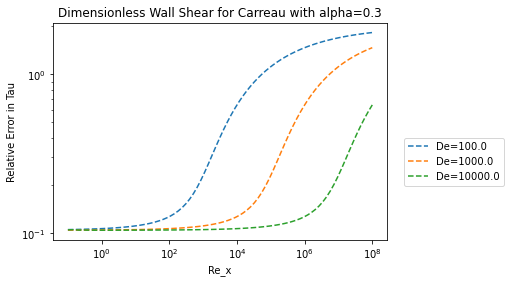
\includegraphics[width=\linewidth]{ws_pt_3_sak.png}
    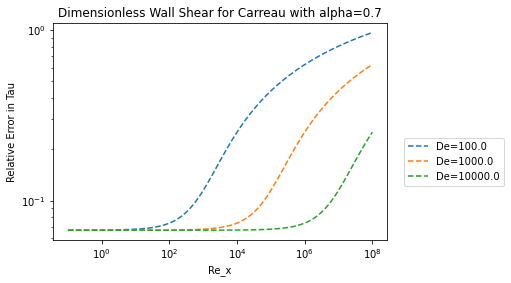
\includegraphics[width=\linewidth]{ws_pt_7_sak.png}
    \caption{Error in wall shear predictions near the front of the plate for $\alpha = 0.3$ (top) and $\alpha = 0.7$ (bottom) for various Deborah numbers. The power-law fluid reproduces the correct asymptotic form of the Carreau wall shear but with a slight error in the asymptotic coefficient that decreases as $\alpha \to 1$.}
    \label{fig:ws_front_err_proof}
\end{figure}

We note that this is consistent with the key identity of the Polhausen approach to wall shear computation, which expresses the wall shear as a global integral of the velocity profile. In the Blasius case, for instance, \begin{equation}
    \bar{\tau}_i = \frac{\text{d}}{\text{d}x} \int_0^\infty u_x(U-u_x) ~ \text{d}y. \label{schlic} \end{equation}

Thus, the global velocity field affects the wall shear. Note that even in the low $\operatorname{Re}_{n, x}$ regime near the front of the plate, the Carreau fluid behavior is Newtonian far enough from the wall. Hence, (\ref{schlic}) indicates that the wall shear may fail to be completely captured by the power-law limit even though that limit describes most of the flow field; this expresses itself in the asymptotic error $c(\alpha)$.

For practical fluids, by the empirically observed monotonicity of $c$ in $\alpha$, the worst-case error is reached for strongly shear-thinning fluids with $\alpha \sim 0.3$. In this regime $c$ is on the order of $0.1$, meaning the worst-case error incurred is approximately $10\%$. In practice, this is not significantly larger in absolute or relative terms than the error incurred near the transition region where the rheology switches from power-law to Newtonian. In the Newtonian region, the Carreau and Newtonian wall shears appear to match asymptotically as $\operatorname{Re}_{n, x} \to \infty$, so this worst-case error is not problematic in most applications. For most practical settings, the self-similar solutions are well-predictive of Carreau wall shear, while for greater accuracy one can still solve the one-parameter family of ODEs (\ref{carreau_ode_form_full_system}) to obtain the full Carreau solution.

\subsection{Velocity Profiles and Broader Observations}

A plot of the wall shears as a function of $\operatorname{Re}_{n,x}$, which scales with the distance along the plate $x$, exhibits the intuitive transition structure described above and is shown in Figure~\ref{fig:wallshearfig}. This behavior maps quite cleanly onto the underlying rheology. At a physical level, it appears that it is the relevant viscosity at the wall, more than the impact of shear-thinning on the velocity profile, that governs the wall shear rate for the Sakiadis and Blasius problems. Capturing the wall-shear behavior does not therefore imply that the full fluid profile is correctly reproduced.

Analysis of the velocity profiles shown in Figures~\ref{fig:profiles}--\ref{fig:profiles3} reveals that there are many instances in which the wall shear prediction is qualitatively good even when the entire velocity profile is not, since the correct gradient needs to be captured only in the vicinity of the wall---though this is still determined by a boundary value problem, so the far-from-wall behavior does have some effect. We note that, while the power-law model provides an accurate description of the Carreau wall shear in the high-shear regime (near the front of the plate), this does not imply that the full power-law predicted velocity profile is accurate for large $\eta$ (far from the plate). After all, the shear prediction requires good resolution of the velocity profile only in the vicinity of the wall.

\begin{figure}
    \centering
    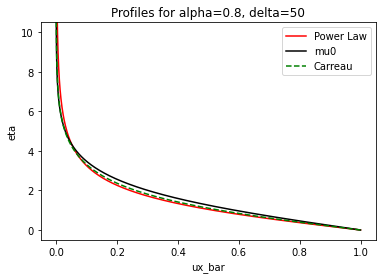
\includegraphics[width=0.8\linewidth]{prof1.png}
    \caption{Velocity profiles for the self-similar and Carreau viscosity models for a typical shear-thinning fluid at an intermediate distance along the wall.}
    \label{fig:profiles}
\end{figure}

\begin{figure}
    \centering
    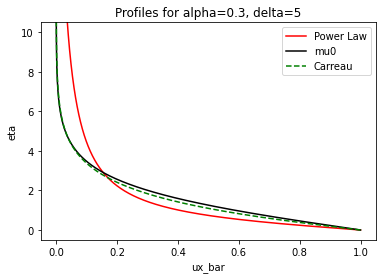
\includegraphics[width=0.8\linewidth]{prof3.png}
    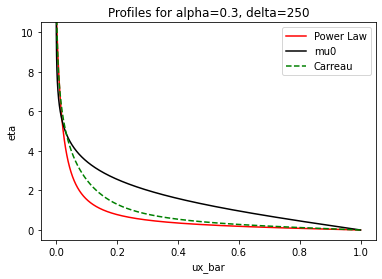
\includegraphics[width=0.8\linewidth]{prof4.png}
    \caption{Velocity profiles for the self-similar and Carreau viscosity models for a strongly shear-thinning Sakiadis flow at two distances along the wall.}
    \label{fig:profiles2}
\end{figure}

\begin{figure}
    \centering
    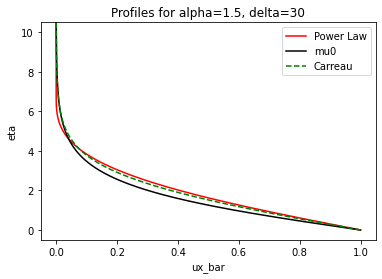
\includegraphics[width=0.4\linewidth]{prof5.png}
        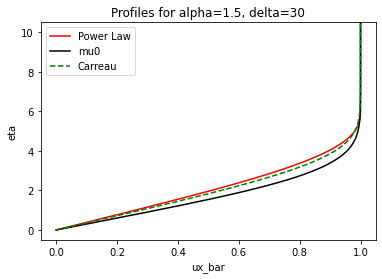
\includegraphics[width=0.4\linewidth]{blas_thick_30 - Copy.png}
    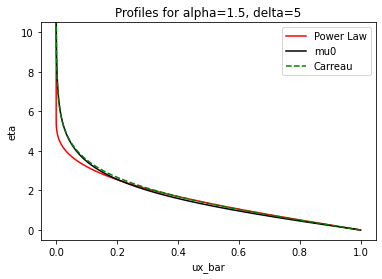
\includegraphics[width=0.4\linewidth]{prof6.png}
        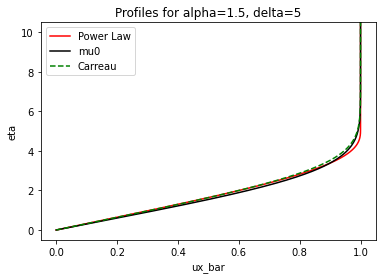
\includegraphics[width=0.4\linewidth]{blas_thick_5 - Copy.png}
    \caption{Velocity profiles for the self-similar and Carreau viscosity models for the shear-thickening Sakiadis problem (left) and the Blasius problem (right) at two distances along the wall.}
    \label{fig:profiles3}
\end{figure}

The profiles in Figures~\ref{fig:profiles}--\ref{fig:profiles3} indicate that the velocity profile from the power-law model is not a perfect estimate for the Carreau fluid even for values of $\delta$ for which the power-law wall shear agrees with the Carreau wall shear. That said, far from the plate and very close to the front of the plate, we note that the fluid streamlines in the Sakiadis and Blasius solutions do not appear to have small slope, indicating that the boundary layer approximation is breaking down in the regime where the power-law solution provides an inaccurate description of the Carreau velocity field. While there does appear to be a region in which the Carreau velocity field is not well-matched by the power-law model while the boundary layer approximation still holds, the full Carreau solution remains physically meaningful in that case and can be directly computed.

We note that the match of wall shears even in regions where the velocity profile agrees less well implies that it is the behavior of the non-Newtonian viscosity $\mu$, rather than the impact of the modified profile on the applied shear $\partial u_x/\partial y$, that has the greater effect on the wall shear of a Carreau boundary layer. We note that this is the \textit{opposite} of the effect that non-Newtonian rheologies have on the stability of laminar boundary layers according to \cite{Griffiths}, which is of some interest, though not particularly surprising given that stability and shear rate correspond to rather different features of the flow field.

We also point out that the inability to take the power-law velocity profiles as accurate representations of the full fluid profile far from the plate is physically consistent with the fact that this is precisely the regime in which the singular behavior of the new solutions takes effect. In some sense, this indicates that the flow far from the plate need not be described with great precision---it is essentially plug flow---but that if one wants precise, quantitative estimates of the full velocity profile of a non-Newtonian fluid in a boundary layer, the Newtonian plateau of the rheology plays a significant role.

We point out the work of Denier and Dabrowski \cite{Dabrowski}, who considered the origin of the breakdown in the solution to the full boundary layer problem for shear-thickening fluids. They point out that this can be seen as a breakdown in the boundary layer equations. For a shear-thickening power-law fluid, the fluid is approximately inviscid far from the wall since the shear is small there. The Carreau solution, which is well-behaved far from the wall, avoids this issue because the fluid viscosity approaches the Newtonian plateau $\mu_0$ in the low-shear limit. This is consistent with Denier and Dabrowski's finding that a continuous solution can be recovered by introducing a ``viscous diffusion layer'' in which viscous effects from shear not normal to the wall become relevant, effectively recovering a more viscous response in that regime. In a broader sense, correcting the non-smoothness in the shear-thickening power-law solution is fundamentally about restoring appropriate viscous behavior in the low-shear limit.

Finally, we note that this also validates the power-law model in the shear-thickening case in a manner analogous to the shear-thinning one. Physically meaningful behavior for any rheological regime is achievable with the Carreau model, and the power-law solution gives an especially good approximation to the Carreau wall shear near the front of the plate, while providing reasonably accurate---though sometimes imperfect---velocity profiles far from the plate.

\section{Conclusion}

The present work investigated the boundary layer flows of a non-Newtonian fluid over a flat plate, focusing on both the Sakiadis and Blasius boundary layers. While the physically realistic Carreau viscosity model does not admit self-similar solutions, the wall shear predictions are well-approximated by the self-similar solutions in the Newtonian and power-law regimes. These regimes can be identified a priori from self-similar calculations alone, and the corresponding predictions were found to match the Carreau flow. The self-similar solutions provided reliable wall shear predictions in each regime, and this framework was found to apply for both the Sakiadis and Blasius flows across a wide range of rheologies. As part of this, for the Sakiadis flow, we showed that solutions exist in a generalized sense for power-law exponents where previous work had concluded no solutions were possible, and that these solutions are consistent with the wall shear predictions in the power-law regime of the Carreau model.


\bibliographystyle{plain} % We choose the "plain" reference style
\bibliography{biblio} % Entries are in the refs.bib file


\end{document}
